\documentclass[polish,bachelor,a4paper,oneside]{ppfcmthesis}

\usepackage[utf8]{inputenc}
\usepackage[OT4]{fontenc}
\usepackage{polski}
\usepackage{mathtools}
\usepackage{graphicx}
\graphicspath{{figures/images/}}
\usepackage{float}
\usepackage{multicol}
\usepackage{subcaption}
\usepackage{listings}


% Authors of the thesis here. Separate them with \and
\author{%
   Jacek Kubiak \album{116307} \and 
   Tomasz Kasperek \album{116393} \and
   Mikołaj Szal \album{117068} \and 
   Paweł Mieloch \album{117077}}
\authortitle{} % Do not change.
\title{Opracowanie systemu automatycznego proponowania odpowiedzi dla nowych pytań na~forach Q\&A} % Note how we protect the final title phrase from breaking
\ppsupervisor{dr~inż.~Agnieszka Ławrynowicz}
\ppguide{mgr~inż.~Dawid Wiśniewski}
\ppyear{2018}

\begin{document}

% Front matter starts here
\frontmatter\pagestyle{empty}%
\maketitle\cleardoublepage%

% Blank info page for "karta dyplomowa"
\thispagestyle{empty}\vspace*{\fill}%
\begin{center}Tutaj przychodzi karta pracy dyplomowej;\\oryginał wstawiamy do wersji dla archiwum PP, w pozostałych kopiach wstawiamy ksero.\end{center}%
\vfill\cleardoublepage%

% Table of contents.
\pagenumbering{Roman}\pagestyle{ppfcmthesis}%
\tableofcontents* \cleardoublepage%

\mainmatter
\chapter{Wstęp}

\section{Uzasadnienie podjęcia tematu}
W internecie coraz większą popularnością cieszą się fora CQA (ang. \textit{Community Question Answering}). Tego typu fora rzadko ograniczają kto i na jaki temat może zadać pytanie lub napisać odpowiedź. W rezultacie użytkownicy mają dużą swobodę publikowania pytań i mogą liczyć na szczere odpowiedzi poparte doświadczeniami innych. Niestety problem stwarza duża liczba udzielonych odpowiedzi. Przeczytanie ich wszystkich może się okazać bardzo czasochłonne. Dodatkowe trudności może też sprawiać zrozumienie skomplikowanych odpowiedzi. Rozwiązaniem tego problemu byłby system automatyzujący proces szukania odpowiedzi.
Stworzenie takiego systemu zostało zaproponowane jako temat jednego z zadań w konkursie SemEval 2017. \cite{SemEval-2017:task3} Konkurs ten jest organizowany co roku pod patronatem grupy SIGLEX (ang. \textit{Special Interest Group on the Lexicon of the Association for Computatnional Linguistics}). 

\section{Cel pracy}
Celem pracy jest stworzenie systemu, który będzie spełniał wymagania określone w zadaniu trzecim konkursu SemEval 2017. Zadanie polega na stworzeniu modeli klasyfikujących, działających na danych charakterystycznych dla forum typu CQA. %(Community Question Answearing).

\section{Zakres pracy}
Zakres pracy obejmuje następujące zadania:
\begin{itemize}
  \item zapoznanie się z podstawowymi metodami przetwarzania języka naturalnego,
  \item zrozumienie podstaw działania modeli uczących, w szczególności sieci neuronowych oraz nabycie umiejętności realizacji takich modeli,
  \item stworzenie modelu klasyfikującego istniejące pytania pod względem podobieństwa do nowego pytania,
  \item stworzenie modelu klasyfikującego istniejące odpowiedzi pod względem użyteczności dla istniejących pytań,
  \item stworzenie modelu klasyfikującego istniejące odpowiedzi pod względem użyteczności dla nowego pytania,
  \item ewaluacja skuteczności każdego z modeli.
\end{itemize}

Ze względu na dopasowanie liczby podzadań w konkursie do liczby osób w zespole realizującym pracę dyplomową, postanowiono przydzielić każdej osobie jedno podzadanie. Dodatkowo, przed przystąpieniem do implementacji, każdy musiał zapoznać się z tematyką przetwarzania języka naturalnego i wchodzącymi w jej skład technikami uczenia maszynowego.
%AL%%% - być może warto wcześniej napisać, że zadanie trzecie w SemEval dzieli się na podzadania A, B,C,D,E, bo bez tego odwołujemy się do tych numerów, o których wcześniej nie było mowy. Być może warto by też było napisać po jednym zdaniu, bardzo skrótowo (jak się uda) na czym polega każde z tych podzadań.  
\begin{center}
\begin{tabular}{ | p{3cm} | p{10cm} | }
 \hline
  Osoba & Zadania \\
 \hline
 Jacek Kubiak & Opanowanie podstawowej wiedzy z zakresu przetwarzania języka naturalnego, realizacja podzadania B \\ 
 \hline
 Tomasz Kasperek & Opanowanie podstawowej wiedzy z zakresu przetwarzania języka naturalnego, realizacja podzadania E \\  
 \hline
 Mikołaj Szal & Opanowanie podstawowej wiedzy z zakresu przetwarzania języka naturalnego, realizacja podzadania C \\
 \hline
 Paweł Mieloch & Opanowanie podstawowej wiedzy z zakresu przetwarzania języka naturalnego, realizacja podzadania A \\
 \hline
\end{tabular}
\end{center}

\section{Źródła}
Jako główne źródło nabywania wiedzy o uczeniu maszynowym posłużyła książka ,,\emph{Hands-On Machine Learning}'' \cite{handson2017}. Dodatkowo wykorzystano kilka artykułów dostępnych w internecie, m.in. artykuł na temat syjamskich sieci neuronowych \cite{malstm:medium}.

\section{Układ pracy}

W drugim rozdziale zostały opisane teoretyczne podstawy, skupiające się na wytłumaczeniu pojęć kluczowych do zrozumienia pracy. W rozdziale trzecim, wyjaśniona została struktura danych oraz treści poszczególnych podzadań. Kolejny rozdział opisuje technologie wykorzystane do zrealizowania pracy. Rozdział piąty to wyjaśnienie wykorzystanych architektur sieci neuronowych oraz szczegółowy opis wykonanych eksperymentów i rezultatów uczenia sieci neuronowych. Ostatni rozdział jest podsumowaniem, przedstawiającym wnioski oraz spostrzeżenia wyniesione z pracy.
\chapter{Wybrane zagadnienia analizy semantycznej języka naturalnego}

Analiza semantyczna jest trudnym zagadnieniem ze względu na złożoność języków naturalnych. Często ich reguły są skomplikowane, zawierają znacznie więcej wyjątków niż języki formalne, które są prostsze w przetwarzaniu komputerowym. Znaczenie poszczególnych wyrazów może być zależne od kontekstu całego zdania bądź akapitu.

\section{Przetwarzanie języka naturalnego}

\subsection{Word Embeddings}
Word Embeddings to jedna z technik przetwarzania języka naturalnego  (ang. \textit{Natural Language Processing, NLP}) służąca do modelowania języka i ekstrahowania informacji z zapisu tekstowego. W dużym uproszeniu, Word Embedding polega na reprezentowaniu znaczeń słów lub zdań jako wielowymiarowe wektory abstrakcyjnych numerycznych cech. Motywacją przemawiającą za wykorzystaniem takiej reprezentacji danych jest fakt, iż komputery nie radzą sobie z analizowaniem tekstu w postaci ciągu znaków. Wartości numeryczne są naturalnym formatem danych wejściowych w większości systemów realizujących algorytmy przetwarzania danych. Metody tworzenia takich powiązań oparte są na statystyce, macierzach współwystąpień (\textit{ang. co-occurence matrix}) i sieciach neuronowych.

\subsubsection{Wektor wystąpień (\textit{ang. Count Vector})}
Rozważmy korpus $C$ składający się z $D$ dokumentów $\{d_1, d_2,..., d_D\}$ i N unikatowych wyrazów wydobytych z korpusu $C$. Niech to $N$ wyrazów jest naszym słownikiem, a rozmiar macierzy wektorów wystąpień to $D \times N$. Każdy wiersz macierzy zawiera częstotliwość wystąpienia wyrazów w dokumencie $d(i)$, gdzie $i = \{1, 2, ... ,D\}$.

\subsubsection{Macierz współwystąpień}
Reprezentacja danych polegająca na zliczeniu wystąpień słów $w1$ i $w2$ w obszarze okna o stałym rozmiarze. Rozważmy korpus $C$ składający się z $N$ unikalnych słów. Macierz wpółwystąpień będzie miała rozmiar $N \times N$. Zaletą macierzy współwystąpień jest zachowanie relacji między słowami, niestety wadą takiej reprezentacji danych jest duże zapotrzebowanie pamięci przy przetwarzaniu większej ilości tekstu.

\subsubsection{CBOW}
CBOW to algorytm tworzący Word Embeddingi z wykorzystaniem sieci neuronowej. CBOW próbuje przewidzieć wystąpienie słowa w kontekście innych słów. Architekura sieci wykorzystanej w algorytmie CBOW składa się z 3 warstw:
\begin{itemize}
  \item Warstwa wejściowa to macierz o rozmiarze $X \times V$ gdzie każdy wiersz to wektor zer i jedynek, w którym wartość 1 oznacza wystąpienie danego słowa w zadanym kontekście. $V$ to liczba unikatowych słów w korpusie,
  \item Warstwa ukryta zbudowana z $N$ neuronów o liniowej funkcji aktywacji,
  \item Warstwa wyjściowa będąca $V$-wymiarowym wektorem prawdopodobieństw wystąpienia słowa w danym kontekście.
\end{itemize}
Aktywacja warstwy ukrytej jest traktowana jako wektorowa reprezentacja zadanego słowa.
Architektura to została zilustrowana na rysunku~\ref{fig:cbow}.
\begin{figure}[H]
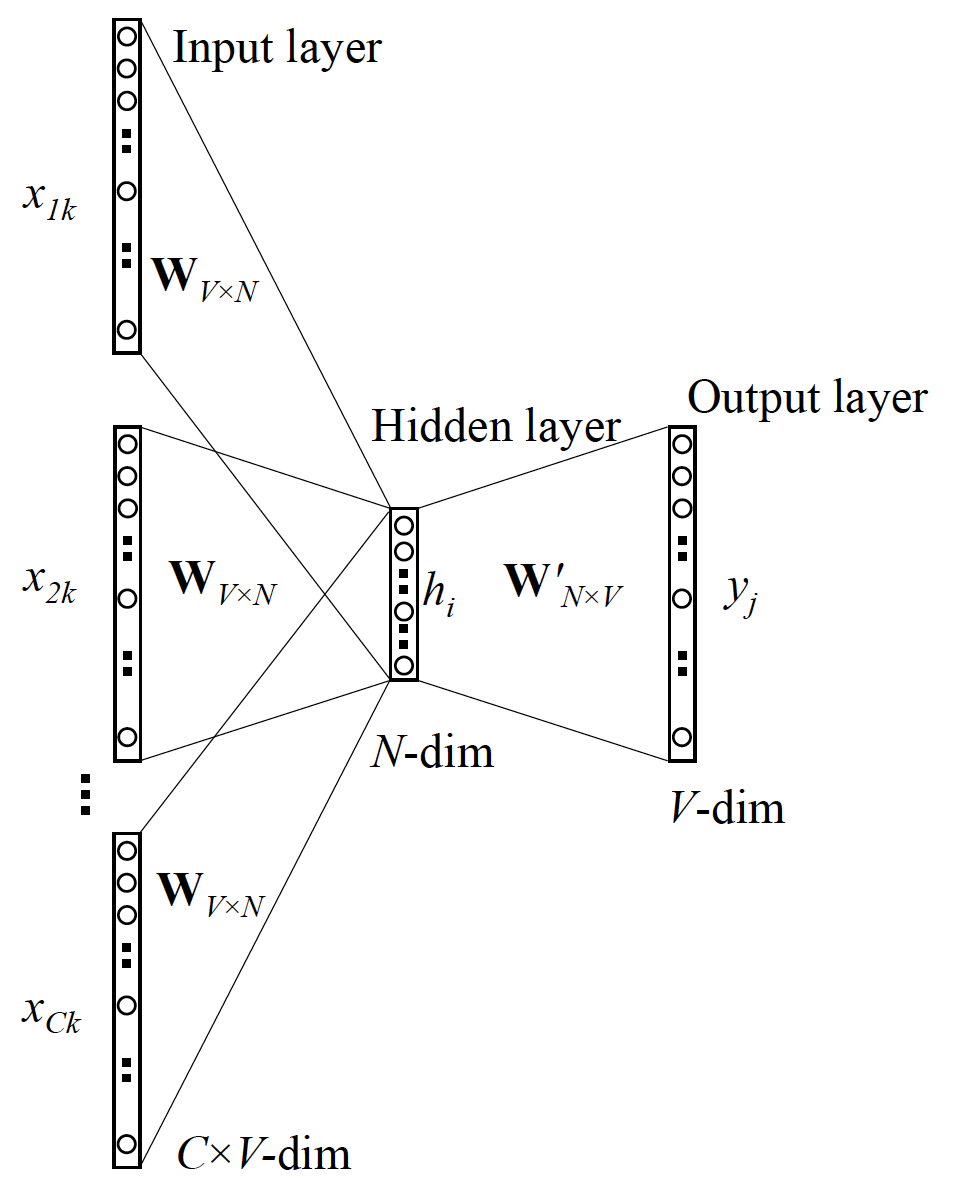
\includegraphics[scale=0.2]{fig-word2vec-cbow}
\centering
\caption{Architekura sieci wykorzystanej w algorytmie CBOW. %AL%%%- źródło?
\label{fig:cbow}}
\end{figure}

\subsection{Miary podobieństwa}

\subsubsection{Indeks Jaccarda}
Indeks Jaccarda to miara oparta na algebrze zbiorów. Wyraża się ją wzorem:
%\[
\begin{equation}
  J(A,B) = \frac{|A \bigcap B|}{|A \bigcup B|}
\end{equation}
%\]

Gdzie:
\begin{itemize}
\item A, B - skończone zbiory
\item $J(A,B)$ - wartość indeksu Jaccarda
\end{itemize}
Wartość indeksu zawiera się w zbiorze $\langle 0,1 \rangle$. Jeżeli oba zbiory są puste, jako wartość indeksu przyjmuje się 1. W przypadku przetwarzania języka, można zastosować tą miarę do wyrażenia podobieństwa dwóch tekstów. Tekst należy w tym celu przedstawić jako zbiór tokenów, czyli rdzeni słów. Dla tak utworzonych zbiorów można zastosować indeks Jaccarda.
Prostota, choć jest niewątpliwą zaletą tej miary, rodzi również pewne problemy. Po pierwsze, reprezentacja w postaci zbioru nie pozwala odzwierciedlić informacji jaką może nieść kolejność słów. Po drugie, nie są uwzględniane synonimy, a zatem dwa teksty o podobnym znaczeniu, ale złożone z różnych wyrazów otrzymają niską wartość podobieństwa.

\subsubsection{Podobieństwo kosinusowe}
Wygodną miarą podobieństwa dla tekstu reprezentowanego w postaci wektorów może być podobieństwo kosinusowe, czyli wartość funkcji kosinus. Taka miara może być użyta dla wektorów o dowolnej liczbie wymiarów. Dodatkowo, dla wektorów z dodatniej przestrzeni będzie przyjmowała wartości z przedziału $\langle 0,1 \rangle$.
Podobnie jak indeks Jaccarda, podobieństwo kosinusowe charakteryzuje prostota. Jednak w tym przypadku, miara operuje na bardziej trafnej reprezentacji tekstu i nie powoduje utraty informacji.

\subsubsection{Długość tekstu}
Inną, prostą metodą określania podobieństwa tekstów może być porównanie długości. Miara, choć naiwna, może niekiedy być użyteczna. Można podejrzewać, że dwa teksty o podobnym znaczeniu będą miały zbliżoną długość, natomiast duże różnice w długości mogą oznaczać znaczną rozbieżność treści. 
W praktyce miara długości okazuje się jednak mało trafna i nie daje zadowalających wyników. 




\chapter{Specyfikacja wymagań}
System powinien realizować cztery główne funkcje, opisane w konkursie Sem-Eval jako podzadania A, B, C oraz E.

\section{Opis danych}
System powinien zostać stworzony w oparciu o dostarczony zbiór danych. Dane pochodzą z forów internetowych Qatar Living oraz Stack Exchange i mają ściśle określoną budowę. Zbiór, wraz z opisem, jest dostępny na stronie konkursu.

\subsection{Dane dla zadań A -- C}
Zbiór danych jest dostarczony w plikach o formacie XML. Zorganizowany jest jako sekwencja oryginalnych pytań (nie zadanych wcześniej na forum), do których jest przypisane po dziesięć wątków. Każdy wątek składa się z pytania powiązanego oraz dziesięciu komentarzy.
Każdy komentarz w wątku posiada dwie etykiety. Pierwsza określa w jakim stopniu komentarz odpowiada na oryginalne pytanie, druga w jakim stopniu odpowiada na pytanie powiązane. Obie te etykiety mogą przyjmować jedną z trzech wartości: ,,Good'', ,,PotentiallyUseful'', ,,Bad''.
Każde powiązane pytanie zawiera natomiast etykietę określającą podobieństwo do oryginalnego pytania. Wartości jakie przyjmuje ta etykieta to: ,,PerfectMatch'', ,,Relevant'', ,,Irrelevant''.

\subsection{Dane dla zadania E}
Zbiór danych dla tego zadania składa się z sekwencji oryginalnych pytań oraz 50 wątków zawierających jedno pytanie powiązane wzbogacone o atrybuty: kategoria, data, tagi, punktacja, liczba wyświetleń, identyfikator użytkownika oraz etykietę:
\begin{itemize}
\item „PerfectMatch'' – informującą o tym, że pytanie prawie całkowicie pokrywa się z pytaniem oryginalnym,
\item „Related'' – informującą, że pytanie zgadza się częściowo z pytaniem oryginalnym,
\item „Irrelevant'' – informującą, że różni się całkowicie od pytania oryginalnego
\end{itemize}.
W wątku może znajdować się również wiele odpowiedzi na pytanie powiązane oraz komentarze zawierające dodatkowe pola tj.: punktację, identyfikator użytkownika oraz datę umieszczenia. Powiązana odpowiedź zawiera również informację o tym, czy została zaakceptowana przez autora pytania.

\section{Zadania systemu}

\subsection{Podzadanie A}
Zadanie polega na wyznaczeniu trafności odpowiedzi na dane pytanie. Mając pytanie oraz pierwszych 10 komentarzy, należy sklasyfikować komentarze biorąc pod uwagę ich związek z tematem pytania. Komentarze posiadające etykietę ,,Good'' powinny trafniej odpowiadać na pytanie niż te z etykietami ,,PotientallyUseful'' i ,,Bad''. Dwie ostatnie etykiety nie są rozróżnialne i mogą zostać sprowadzone do jednej.

\subsection{Podzadanie B}
Zadanie polega na wyznaczeniu podobieństwa między dwoma pytaniami. Mając nowe pytanie oraz zbiór 10 powiązanych pytań, należy sklasyfikować powiązane pytania, biorąc pod uwagę ich związek z nowym pytaniem. Pytania z etykietami ,,PerfectMatch'' oraz ,,Relevant'' są uznawane za równie dobre, nie rozróżniamy ich. Powinny mieć wyższe podobieństwo od tych z etykietą ,,Irrelevant''.

\subsection{Podzadanie C}
Zadanie polega na wyznaczeniu dla pytania najbardziej trafnych odpowiedzi, które pochodzą z różnych wątków. Mając nowe pytanie (nazwijmy to głównym pytaniem) i zbiór powiązanych pytań (pierwsze 10) - każde  wraz z odpowiedziami (pierwszymi 10-cioma), należy sklasyfikować tych 100 odpowiedzi biorąc pod uwagę ich związek z głównym pytaniem. Komentarze z etykietą ,,Good'' powinny trafniej odpowiadać na pytanie niż komentarze z etykietą ,,PotentiallyUseful'' lub ,,Bad''. Ostatnie dwie etykiety uznane są za identyczne i zostały zredukowane do jednej.

\subsection{Podzadanie E}
Podzadanie E polega na detekcji zduplikowanych pytań. 50 potencjalnie zduplikowanych pytań należy sklasyfikować mając na względzie ich podobieństwo do zadanego pytania. Następnie należy usunąć ze zbioru pytania, tak aby ostateczny rezultat zawierał wyłącznie pytania z etykietą ,,PerfectMatch''. Pytania z etykietami ,,Related'' oraz ,,Irrelevant'' powinny zostać pominięte.

\chapter{Technologie}
Przed rozpoczęciem pracy należało rozważyć wybór technologii do zrealizowania algorytmów uczenia maszynowego rozwiązujących przedstawione problemy. Do implementacji został wybrany język Python ze względu na największy dostęp bibliotek związanych z analizą danych i uczeniem maszynowym. Język ten cieszy się ogromną popularnością wśród społeczności inżynierów danych, co również przeważyło na jego korzyść. Do zaimplementowania sieci neuronowej wykorzystano bibliotekę TensorFlow wraz z wysokopoziomową nakładką Keras. Dodatkowo użyto kilku bibliotek pomocniczych takich jak NLTK i Gensim. Wykorzystano również wcześniej wytrenowane word-embeddingi pochodzące ze zbioru GoogleNews-word2vec.

\section{TensorFlow}
TensorFlow \cite{tensorflow2015-whitepaper} to biblioteka o otwartych kodach źródłowych (ang. \textit{open source}) służąca do wykonywania obliczeń numerycznych z wykorzystaniem grafów przepływów danych. Elastyczna architektura ułatwia komunikację między CPU i GPU za pomocą jednego API. TensorFlow jest rozwijany przez Google Brain Team w celu rozwoju badań nad uczeniem maszynowym i głębokimi sieciami neuronowymi.

\section{Keras}
Keras \cite{keras} to wysokopoziomowe API umożliwiające łatwe i wygodne programowanie sieci neuronowych. Keras może korzystać z różnych silników obliczeniowych między innymi z TensorFlow. Wspiera on sieci konwolucyjne, rekurencyjne, a nawet bardziej zaawansowane modele takie jak np. sieci syjamskie. 

\section{NLTK}
NLTK (ang. \textit{Natural Language Toolkit})~\cite{nltk} to przodująca platforma do budowania programów przetwarzających dane związane z językiem naturalnym. Udostępnia łatwy w użyciu interfejs pozwalający wykonywać zadania związane z przetwarzaniem tekstu, takie jak klasyfikacja, tokenizacja lub parsowanie.

\section{Gensim}
Gensim \cite{rehurek_lrec} jest jedną z wydajniejszych i prostszych w użyciu bibliotek realizujących nienadzorowane modelowanie semantyczne na podstawie czystego tekstu. Gensim został wykorzystany do obsługi wcześniej wytrenowanych embeddingów pochodzących z bazy GoogleNews-word2vec. 

\section{GoogleNews-word2vec}
Publiczna baza word-embeddingów wytrenowanych na podstawie części dokumentów ze zbioru danych Google News. Model zawiera 300 wymiarowe wektory dla ponad 3 milionów słów.

\chapter{Implementacja}

\section{Wykorzystywane modele}
Ze względu na podobieństwa między zadaniami, pewne fragmenty implementowanych modeli powtarzają się. W tym podrozdziale opisano rodzaje sieci neuronowych, które były w projekcie wykorzystywane najczęściej. Są to rozwiązania często realizowane w dziedzinie przetwarzania języka naturalnego.

\subsection{Prosta sieć neuronowa}
Podstawowa architektura sieci neuronowej opiera się na kolejno połączonych ze sobą warstwach neuronów. Warstwy są łączone w sposób szeregowy, najczęściej w oparciu o zasadę ,,każdy z każdym''. Oznacza to, że wyjścia danej warstwy trafiają dalej do wejść każdego z neuronów warstwy następnej. Za wyjątek można uznać pierwszą i ostatnią warstwę sieci. Te warstwy, nazywane wejściową i wyjściową, mają za zadanie doprowadzić dane wejściowe do sieci i wyprowadzić dane wynikowe jako wyjście. Taki model sieci jest wszechstronny i nieskomplikowany, stanowi dobry punkt wyjścia dla rozwiązań z dziedziny uczenia maszynowego. 

\subsection{Sieci rekurencyjne}
Bardziej złożony model, odpowiedni dla danych sekwencyjnych, stanowi sieć rekurencyjna. Tego typu model posiada swego rodzaju pętle zwrotne. Są to połączenia, które doprowadzają do sieci jej własne wyjście. W praktyce stosuje się najczęściej pojedyncze warstwy rekurencyjne. Pętle w sieci rekurencyjnej pozwalają uzyskać pewną właściwość sieci, którą można by nazwać ,,pamięcią''. Oznacza to, że wyniki przeszłych obliczeń wpływają na obliczenia aktualne. Łatwo zauważyć, że takie działanie sieci imituje ludzki sposób analizy sekwencyjnych danych, np. filmu lub tekstu. Ze względu na tę właściwość, sieci (warstwy) rekurencyjne są powszechnie używane w przetwarzaniu języka naturalnego.

\subsection{Sieci syjamskie} \label{arch:malstm}
Przykładem jednej z nowszych architektur wykorzystywanych w przetwarzaniu języka jest sieć syjamska \cite{malstm:paper}. Podstawową cechą takiej sieci jest wprowadzenie dwóch identycznych podsieci, które posiadają osobne wejścia i wyjścia. Taki podział ścieżek przetwarzania pozwala na uzyskanie mechanizmu porównywania danych wprowadzanych na wejścia podsieci. W modelu ogólnym, obie podsieci, choć zbudowane z tych samych elementów, nie mają wspólnych wag i stanowią osobne byty. W trakcie uczenia każda podsieć może przez to nabrać nieco innych właściwości. Do pewnych celów wykorzystuje się jednak sieci syjamskie, w których wagi lub całe warstwy są współdzielone przez podsieci. Model ogólny może być odpowiedni, kiedy pary danych wprowadzane na wejście sieci syjamskiej różnią się pod pewnymi względami. Przykładem z dziedziny przetwarzania języka naturalnego może być porównywanie treści zapytania, podanej przez użytkownika w wyszukiwarce internetowej, z wybraną odpowiedzią. Zapytanie to zazwyczaj kilka słów, które niekoniecznie tworzą zdanie. Odpowiedź wybrana jako stosowna może być jednak dłuższym i bardziej złożonym tekstem. W takim przypadku ważne jest umożliwienie każdej podsieci nabycie własnych wag w procesie uczenia. W innym przypadku, na przykład porównując pary komentarzy z forum internetowego, korzystniejsze jest stworzenie współdzielonych przez podsieci warstw. Pozwala to przyspieszyć proces uczenia bez obniżania skuteczności modelu.
\section{Podzadanie A}
\subsection{Rozkład danych}
Celem podzadania A było wyznaczenie trafności odpowiedzi na pytanie. Z dostarczonego zbioru danych udało się uzyskać ~30 000 przykładów uczących w postaci par pytanie-odpowiedź o różnych etykietach wyrażających trafność odpowiedzi na zadane pytanie. 
Aby uzyskać pewność, że model będzie sobie radził z nowymi danymi wykorzystano metodę statystyczną zwaną sprawdzianem krzyżowym. Zbiór danych został losowo podzielony na zbiór uczący i walidujący w proporcji 4:1. Pozwoliło to uzyskać ~24000 przypadków uczących i ~6000 przypadków walidujących. Po połączeniu klas ,,PotentiallyUseful'' i ,,Bad'' w jedną klasę ,,Bad'' rozkład etykiet w obu zbiorach był następujący:

\begin{table}[H]
\caption{Rozkład klas w zbiorze uczącym}
\label{train_set_statistics_score_table}
    \begin{center}
        \begin{tabular}{ |c|c| } 
            \hline
            klasa & rozkład\\
            \hline
            ,,Good'' & 36,951\% \\
            \hline
            ,,Bad'' & 63,049\% \\
            \hline
        \end{tabular}
    \end{center}
\end{table}

\begin{table}[H]
\caption{Rozkład klas z zbiorze walidującym}
\label{train_set_statistics_score_table}
    \begin{center}
        \begin{tabular}{ |c|c| } 
            \hline
            klasa & rozkład\\
            \hline
            ,,Good'' & 36,277\% \\
            \hline
            ,,Bad'' & 63,723\% \\
            \hline
        \end{tabular}
    \end{center}
\end{table}
\subsection{Miary statystyczne}
W celu rozwiązania problemu klasyfikacji podjęto próby wykorzystania wcześniej zdefiniowanych miar statystycznych. Pierwszą próbą było sprawdzenie zależności między wartością bezwzględną różnicy długości odpowiedzi i pytania, a stopniem trafności odpowiedzi na pytanie (rysunek~\ref{fig:mstatystyczna}).


\begin{figure}[H]
\caption{Zależność różnicy długości i klasy. \label{fig:mstatystyczna}}
\centering
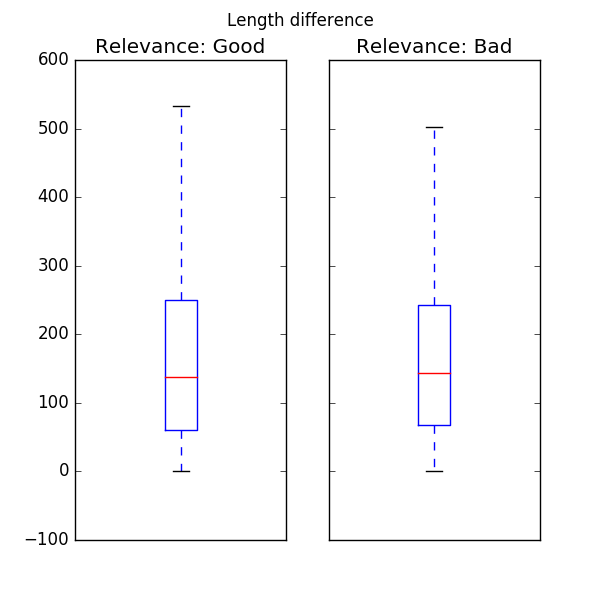
\includegraphics[scale=0.5]{subtask_a_length_difference.png}
\end{figure}

Wartości mediany, pierwszego kwartylu, trzeciego kwartylu są do siebie bardzo zbliżone dla obu wykresów. Również wartości minimalne i maksymalne wykazują podobne wartości. Widać że nie ma większej zależności pomiędzy różnicą długości tekstów, a ich klasą trafności. 
Następną sprawdzoną metryką była zależność pomiędzy indeksem Jaccarda, a trafnością odpowiedzi (rysunek~\ref{fig:jaccarda}). 



\begin{figure}[H]
\caption{Zależność odległości Jaccarda i klasy. \label{fig:jaccarda}}
\centering
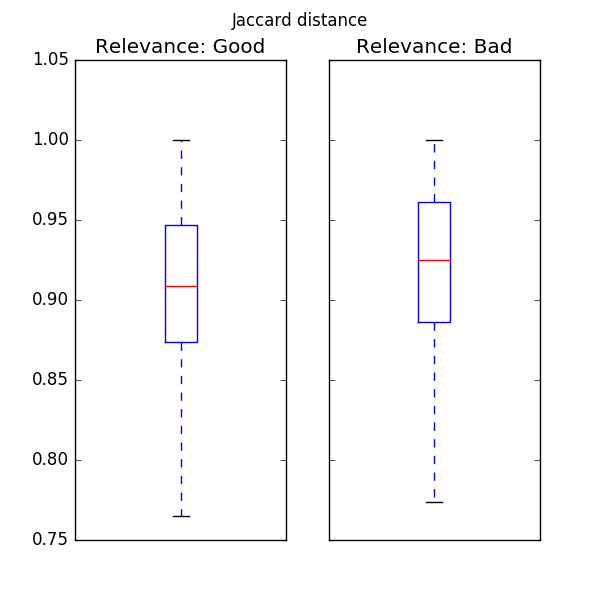
\includegraphics[scale=0.5]{subtask_a_jaccard_distance.png}
\end{figure}

Odnotowano nieznaczne różnice pomiędzy wartościami kwartylu dla obu klas trafności. Różnice pokrywają się z naturą odległości Jaccarda która powinna być większa dla mniej podobnych zbiorów. Widać, że dla klasy ,,BAD'' wartości kwartyli są większe.
  
Ostatnią wykorzystaną metryką była zależność pomiędzy odległością cosinusową, a trafnością odpowiedzi (rysunek~\ref{fig:trafsnosca}). 



\begin{figure}[H]
\caption{Zależność podobieństwa kosinusowego i klasy. \label{fig:trafsnosca}}
\centering
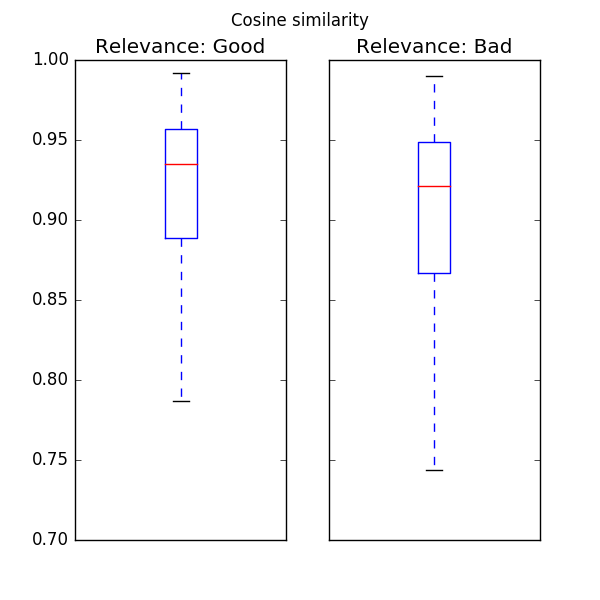
\includegraphics[scale=0.5]{subtask_a_cosine_similarity.png}
\end{figure}

W tym przypadku również wykazano nieznaczne różnice pomiędzy wartościami kwartylu dla obu klas trafności. Różnice pokrywają się z naturą podobieństwa cosinusowego które powinno być większa dla bardziej podobnych zbiorów. Widać że dla klasy ,,GOOD'' wartości kwartyli są większe. 

Na podstawie opracowanych miar statystycznych stworzono klasyfikator oparty na regresji logistycznej (tablice~\ref{tab:train_set_statistics_score_table} i \ref{tab:train_set_statistics_score_table}). Niestety skuteczność tego rozwiązania nie była zadowalająca.

\begin{table}[H]
\caption{Skuteczność regresji logistycznej na zbiorze uczącym. \label{tab:train_set_statistics_score_table}}
    \begin{center}
        \begin{tabular}{ |c|c| } 
            \hline
            metryka & wartość\\
            \hline
            Accuracy & 0,633 \\
            \hline
            Precission & 0,660 \\
            \hline
            Recall & 0,009 \\ 
            \hline
        \end{tabular}
    \end{center}
\end{table}

\begin{table}[H]
\caption{Skuteczność regresji logistycznej na zbiorze walidującym. \label{tab:train_set_statistics_score_table}}
    \begin{center}
        \begin{tabular}{ |c|c| } 
            \hline
            metryka & wartość\\
            \hline
            Accuracy & 0,626 \\
            \hline
            Precission & 0,760 \\
            \hline
            Recall & 0,010 \\ 
            \hline
        \end{tabular}
    \end{center}
\end{table}



\subsection{Prosta sieć feed-forward}

W wyniku małej skuteczności rozwiązań opartych na statystyce podjęto pracę nad bardziej skomplikowanymi modelami - sieciami neuronowymi. Wypróbowano podstawową architekturę jaką jest sieć feed-forward. Składała się ona z jednej w pełni połączonej warstwy ukrytej o rozmiarze 64 jednostek. Na potrzeby wykorzystania sieci neuronowej potrzebna była reprezentacja zdania w formie wektorowej. Każde zdanie zostało zamienione w wektor według wzoru:

%\[
\begin{equation}
\overrightarrow{V} = \frac{\sum_{i=1}^{n}\overrightarrow{s_i}}{n}
\end{equation}
%\]
Gdzie:
\begin{itemize}
\item $n$ - liczba słów w zdaniu,
\item $s$ - word-embedding dla $i$-tego słowa,
\item $V$ - wektorowa reprezentacja zdania.
\end{itemize}

Wejściem sieci były dwa wektory (pytanie i komentarz) połączone w jeden. Wyjściem sieci był pojedynczy neuron wyrażający wyliczoną przez sieć trafność pytania dla odpowiedzi (zob. rysunek~\ref{fig:ffa}).


\begin{figure}[H]
\caption{Architektura sieci. \label{fig:ffa}}
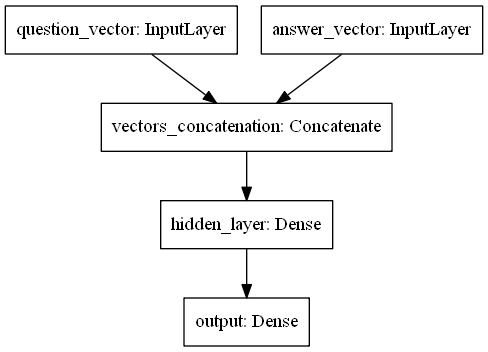
\includegraphics[scale=0.4]{subtask_a_feedforward_model}
\centering
\end{figure}

Sieć zostałą przeuczona zbiorem trenującym, a następnie jej skutecznośc została sprawdzona zbiorem walidującym. Poniżej wykres przedstawiający przebieg uczenia dla 400 epok (rysunki~\ref{fig:ffloss} i \ref{fig:ffacc}).

\begin{figure}[H]
\caption{Przebieg uczenia dla 400 epok (strata). \label{fig:ffloss}}
\centering
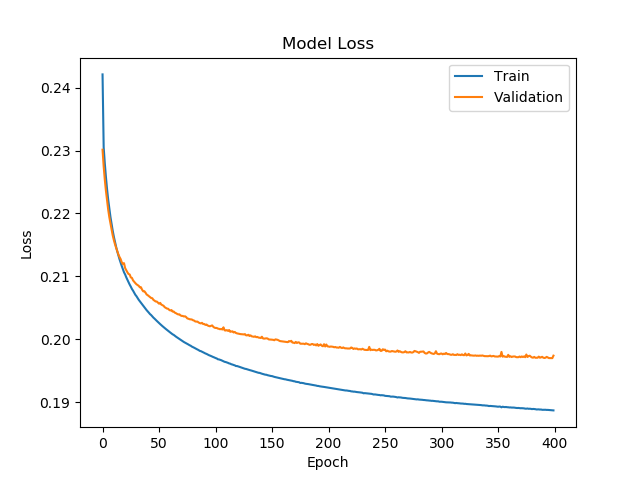
\includegraphics[scale=0.7]{subtask_a_feedforward_loss.png}
\end{figure}


\begin{figure}[H]
\caption{Przebieg uczenia dla 400 epok (trafność). \label{fig:ffacc}}
\centering
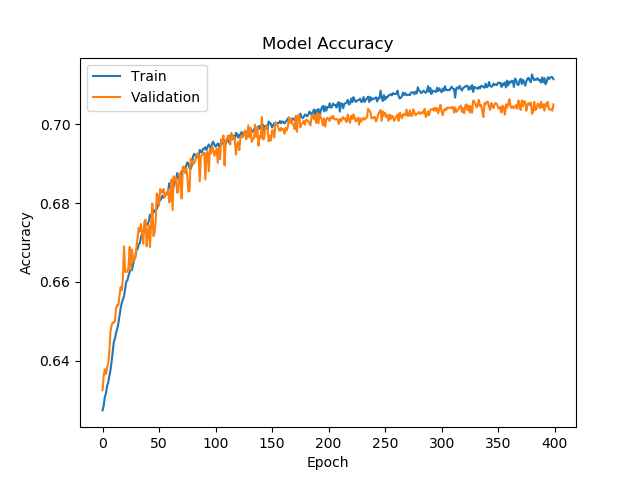
\includegraphics[scale=0.7]{subtask_a_feedforward_acc.png}
\end{figure}




\begin{table}[H]
\caption{Skuteczność sieci feedforward na zbiorze uczącym.\label{tab:ffu}}
\label{train_set_statistics_score_table}
    \begin{center}
        \begin{tabular}{ |c|c| } 
            \hline
            metryka & wartość\\
            \hline
            Accuracy & 0,716 \\
            \hline
            Precision & 0,667 \\
            \hline
            Recall & 0,460 \\ 
            \hline
        \end{tabular}
    \end{center}
\end{table}

\begin{table}[H]
\caption{Skuteczność sieci feedforward na zbiorze walidującym.\label{tab:ffw}}
\label{train_set_statistics_score_table}
    \begin{center}
        \begin{tabular}{ |c|c| } 
            \hline
            metryka & wartość\\
            \hline
            Accuracy & 0,705 \\
            \hline
            Precision & 0,449 \\
            \hline
            Recall & 0,633 \\ 
            \hline
        \end{tabular}
    \end{center}
\end{table}


Rozwiązanie okazało się skuteczne, udało się zwiększyć trafność klasyfikacji o kilka procent (tablice~\ref{tab:ffu} i \ref{tab:ffw}). 


\subsection{Sieć syjamska}

Ostatnią realizowaną architekturą była dużo bardziej skomplikowana sieć syjamska. Posiadała ona dwa wejścia, dwie rekurencyjne warstwy ukryte i warstwę wyjścia. Każdym wejściem była macierzowa reprezentacja zdania. Wierszami macierzy były wektorowe reprezentacje słów występujących w zdaniach. Z powodów technicznych macierze musiały mieć długość równą długości najdłuższego zdania. Dla krótszych zdań były dopisywane wektory zawierające same zera, w celu wyrównania liczby wierszy. Dwie niezależne warstwy rekurencyjne miały za zadanie przekodowania sekwencji wektorów reprezentujących słowa w pojedynczy wektor zawierający semantyczne znaczenie zdania. Jedna warstwa rekurencyjna przetwarzała pytania, a druga odpowiedzi. Następnie te dwa wektory były ze sobą porównywane miarą zwaną odległością manhattańską. Architekturę sieci przedstawiono na rysunku~\ref{fig:acrchrr}.   

\begin{figure}[H]
\caption{Architektura sieci syjamskiej. \label{fig:acrchrr}}
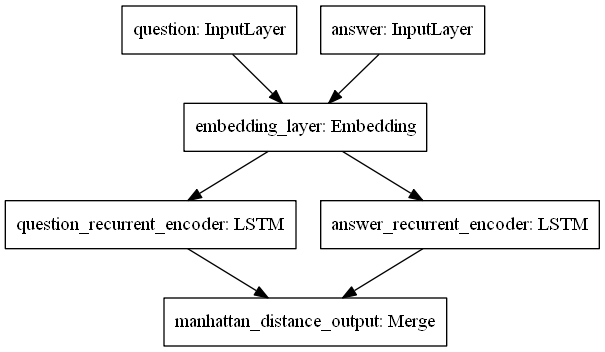
\includegraphics[scale=0.4]{subtask_a_recurrent_model}
\centering
\end{figure}

Sieć została również przeuczona zbiorem trenującym, a następnie jej skuteczność została sprawdzona zbiorem walidującym. Poniżej zamieszczono wykresy przedstawiający przebieg uczenia dla 100 epok (rysunki~\ref{fig:fflossrr} i \ref{fig:ffaccrr}).

\begin{figure}[H]
\centering
\caption{Przebieg uczenia sieci syjamskiej dla 100 epok (strata). \label{fig:fflossrr}}
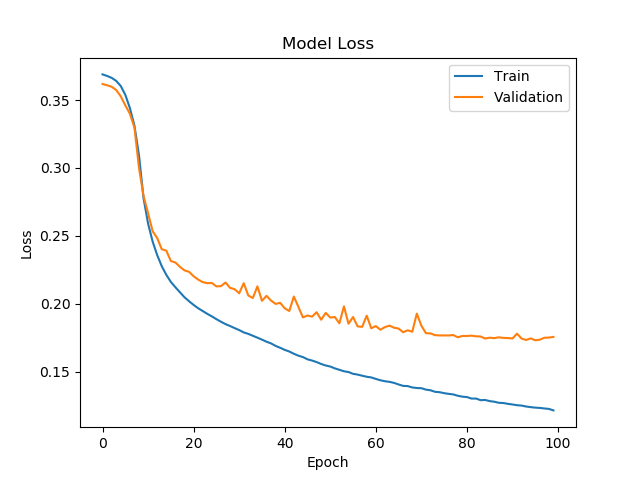
\includegraphics[scale=0.7]{subtask_a_recurrent_loss.png}
\end{figure}


\begin{figure}[H]
\centering
\caption{Przebieg uczenia  sieci syjamskiej  dla 100 epok (trafność). \label{fig:ffaccrr}}
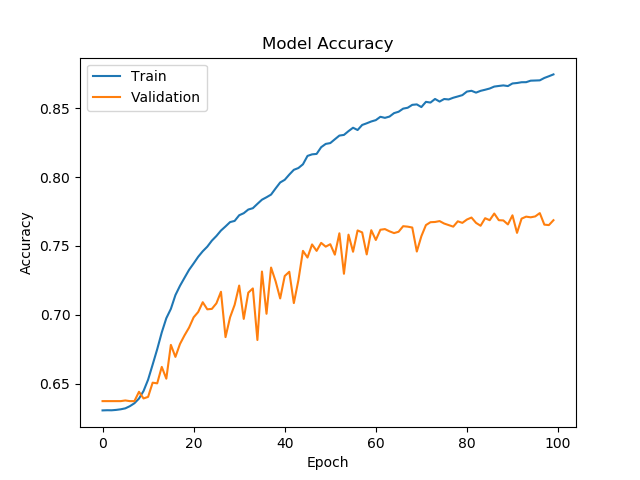
\includegraphics[scale=0.7]{subtask_a_recurrent_acc.png}
\end{figure}


\begin{table}[H]
\caption{Skuteczność sieci syjamskiej na zbiorze uczącym.}
\label{train_set_statistics_score_table}
    \begin{center}
        \begin{tabular}{ |c|c| } 
            \hline
            metryka & wartość\\
            \hline
            Accuracy & 0,883 \\
            \hline
            Precision & 0,877 \\
            \hline
            Recall & 0,796\\ 
            \hline
        \end{tabular}
    \end{center}
\end{table}

\begin{table}[H]
\caption{Skuteczność sieci syjamskiej na zbiorze testowym.}
\label{train_set_statistics_score_table}
    \begin{center}
        \begin{tabular}{ |c|c| } 
            \hline
            metryka & wartość\\
            \hline
            Accuracy & 0,768 \\
            \hline
            Precision & 0,589 \\
            \hline
            Recall & 0,721 \\ 
            \hline
        \end{tabular}
    \end{center}
\end{table}

\subsection{Rozszerzenie zbioru danych}
Jednym ze sposobów zwiększenia skuteczności modeli opartych o uczenie maszynowe jest wytrenowanie ich na większej ilości danych. Niestety nie było możliwości pozyskania nowych przykładów uczących. Problem ten rozwiązano techniką polegającą na sztucznym powiększeniu zbioru danych o nowe przypadki. Na podstawie oryginalnego zbioru został stworzony zbiór rozszerzony, w którym nowe próbki utworzono zamieniając niektóre wyrazy na ich synonimy. 
Dokładną charakterystykę zbioru oryginalnego i rozszerzonego przedstawia tablica~\ref{a_augmented_set_percentage}.

\begin{table}[H]
\caption{Rozkłady ilościowe klas w zbiorze oryginalnym i rozszerzonym.}
\label{a_augmented_set_percentage}
    \begin{center}
        \begin{tabular}{ |c|c|c|c| } 
            \hline
            Zbiór & Liczność zbioru & ,,Good'' & ,,Bad''\\
            \hline
            Oryginalny & 30242 & 36,27\% & 63,04\%\\
            \hline
            Rozszerzony & 124368 & 35.76\% & 64,24\%\\ 
            \hline
        \end{tabular}
    \end{center}
\end{table}

Na zbiorze rozszerzonym został wytrenowany wcześniej przedstawiony model sieci syjamskiej. Wyniki przedstawiają rysunki~\ref{a_siamese_augmented_acc} i \ref{a_siamese_augmented_loss}.

\begin{figure}[H]
\centering
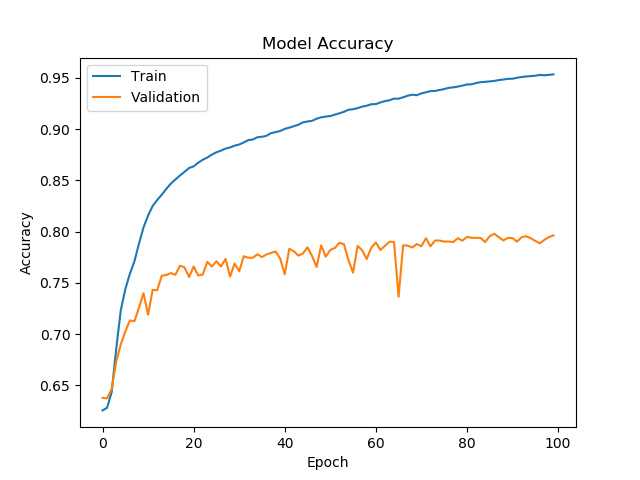
\includegraphics[scale=0.5]{subtask_a_recurrent_augmented_acc}
\caption{Trafność sieci syjamskiej na zbiorze rozszerzonym.}
\label{a_siamese_augmented_acc}
\end{figure}

\begin{figure}[H]
\centering
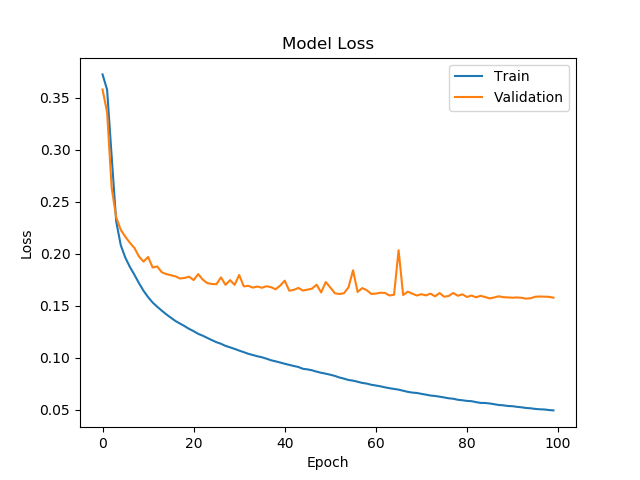
\includegraphics[scale=0.5]{subtask_a_recurrent_augmented_loss}
\caption{Strata sieci syjamskiej na zbiorze rozszerzonym.}
\label{a_siamese_augmented_loss}
\end{figure}


\begin{table}[H]
\caption{Skuteczność sieci syjamskiej na zbiorze rozszerzonym.}
\label{train_set_statistics_score_table_augmented}
    \begin{center}
        \begin{tabular}{ |c|c| } 
            \hline
            metryka & wartość\\
            \hline
            Accuracy & 0.955 \\
            \hline
            Precision & 0.955 \\
            \hline
            Recall & 0.923\\ 
            \hline
        \end{tabular}
    \end{center}
\end{table}

\begin{table}[H]
\caption{Skuteczność sieci syjamskiej na zbiorze testowym.}
\label{train_set_statistics_score_table_augmented}
    \begin{center}
        \begin{tabular}{ |c|c| } 
            \hline
            metryka & wartość\\
            \hline
            Accuracy & 0.796 \\
            \hline
            Precision & 0.633 \\
            \hline
            Recall & 0.764 \\ 
            \hline
        \end{tabular}
    \end{center}
\end{table}

Trafność działania modelu na zbiorze walidującym została zwiększona, osiągnęła ostatecznie wynik około 79\%.

\subsection{Ocena rezultatów}
Analizując wyniki otrzymane po wyuczeniu modelu sieci syjamskiej można stwierdzić że wykorzystanie rozszerzonego zbioru danych podnosi jakość klasyfikacji. Trafność wzrosła z 76.8\% do 79.6\% co stanowi redukcję błędu o 12\%.
\section{Podzadanie B}
\subsection{Rozkład danych}
\subsubsection{Rozkład wartości etykiet}

Podzadanie B miało na celu określenie podobieństwa pomiędzy istniejącym a nowym pytaniem. Pytania posiadały trzy etykiety określające stopień podobieństwa: ,,PerfectMatch'', ,,Relevant'' i ,,Irrelevant''. Rozkład etykiet w oryginalnym zbiorze został przedstawiony w tablicy 5.9.

\begin{table}[H]
\caption{Rozkład klas w oryginalnym zbiorze}
\label{subtask_b_original_set_statistics_score_table}
    \begin{center}
        \begin{tabular}{ |c|c| } 
            \hline
            ,,PerfectMatch'' & 9,28\% \\
            \hline
            ,,Relevant'' & 31,65\% \\
            \hline
            ,,Irrelevant'' & 59,07\% \\ 
            \hline
        \end{tabular}
    \end{center}
\end{table}

Etykiety ,,PerfectMatch'' i ,,Relevant'' zostały określane jako równoważne, w związku z czym zredukowano liczbę etykiet do dwóch, o następujących nazwach: ,,Relevant'' i ,,Irrelevant''. Dodatkowo, cały zbiór podzielono losowo na podzbiór treningowy i walidujący w proporcjach 4:1. Tablice 5.10 oraz 5.11 przedstawiają rozkład klas w utworzonych podzbiorach.

\begin{table}[H]
\caption{Rozkład klas w zbiorze treningowym.}
\label{subtask_b_train_set_statistics_score_table}
    \begin{center}
        \begin{tabular}{ |c|c| } 
            \hline
            ,,Relevant'' & 40,83\% \\
            \hline
            ,,Irrelevant'' & 59,17\% \\ 
            \hline
        \end{tabular}
    \end{center}
\end{table}

\begin{table}[H]
\caption{Rozkład klas w zbiorze treningowym.}
\label{subtask_b_validation_set_statistics_score_table}
    \begin{center}
        \begin{tabular}{ |c|c| } 
            \hline
            ,,Relevant'' & 41,33\% \\
            \hline
            ,,Irrelevant'' & 58,67\% \\ 
            \hline
        \end{tabular}
    \end{center}
\end{table}

Liczność etykiet różni się minimalnie pomiędzy wydzielonymi pozbiorami. W obu można zauważyć przewagę liczności etykiet ,,Irrelevant'' nad etykietami ,,Relevant'', jednak ciężko stwierdzić, aby doszło znacznej skośności danych.

\subsection{Analiza danych}

W ramach wstępnej analizy danych i zdobycia poglądowej wiedzy na temat zbioru danych wykonane zostały obliczenia powszechnych miar statystycznych stosowanych w przetwarzaniu języka naturalnego takich jak: indeks Jaccarda, podobieństwo kosinusowe oraz różnica długości tekstu. Następnie wyniki przedstawiono z podziałem na rodzaj etykiety (rysunek~\ref{fig:lenghtb}).

\begin{figure}[H]
\caption{Zależność różnicy długości i etykiety.\label{fig:lenghtb}}
\centering
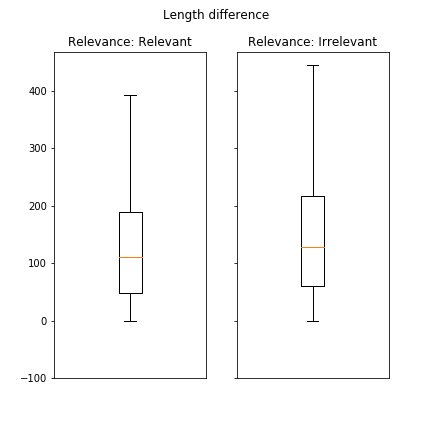
\includegraphics[scale=0.5]{subtask_b_length_difference.png}
\end{figure}

Dla pytań z etykietą ,,Relevant'' wartości maksymalne oraz mediana są mniejsze od pytań z etykietą ,,Irrelevant''. Poza tym, nie występują inne znaczące różnice.

\begin{figure}[H]
\caption{Zależność odległości Jaccarda i etykiety. \label{fig:Jaccardb}}
\centering
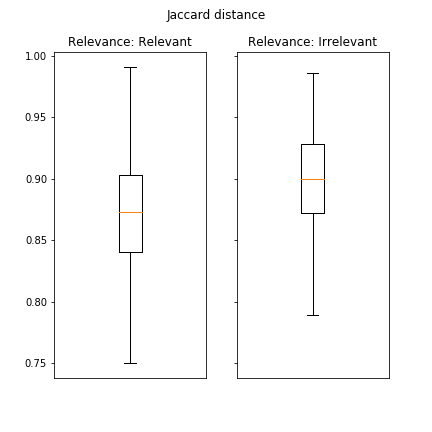
\includegraphics[scale=0.5]{subtask_b_jaccard_distance.png}
\end{figure}

W przypadku odległości Jaccarda pytania z etykietą Relevant uzyskiwały mniejsze wartości mediany (rysunek~\ref{fig:Jaccardb}). Prawie połowa rezultatów zawarła się w zakresie od 0,85 do 0,90, gdzie dla pytań ,,Irrelevant'' były to wartości od 0,88 do 0,93.

\begin{figure}[H]
\caption{Zależność podobieństwa kosinusowego i etykiety. \label{fig:cosinusb}}
\centering
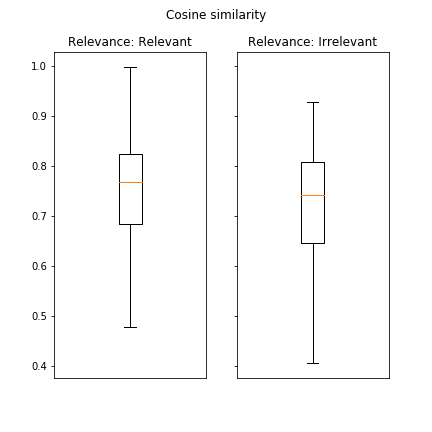
\includegraphics[scale=0.5]{subtask_b_cosine_similarity.png}
\end{figure}

W ostatnim przypadku obliczono podobieństwo kosinusowe i tak jak w przypadku poprzednich miar nie zauważono wyraźnej zależności pomiędzy etykietą a wynikami. Mediana dla ,,Relevant'' była nieznacznie większa od mediany ,,Irrelevant'' (rysunek~\ref{fig:cosinusb}).


\subsection{Sieć rekurencyjna}
\subsubsection{Rezultaty dla pierwotnego zbioru danych}

Aby umożliwić wydajną naukę sieci neuronowej, dane zostały przetworzone do nowego formatu. Oryginalnie pytanie było podzielone na tytuł i korpus. Okazało się jednak, że korpus często zawierał powtórzone pytanie. Stąd decyzja o odrzuceniu tytułu i reprezentowaniu pytania wyłącznie przez korpus. Ponieważ zadaniem była klasyfikacja binarna, zamiast etykiet ,,Relevant'' i ,,Irrelevant'', utworzono jedną etykietę o nazwie ,,Relevance'', która przyjmowała wartość 0 dla ,,Irrelevant'' i 1 dla ,,Relevant''.

Wykorzystana sieć neuronowa była siecią syjamską. Posiadała dwa wejścia, każde z nich przyjmowało wektor indeksów słów występujących w zbiorze treningowym. W kolejnej warstwie elementy wektora wejściowego były przekształcane do word-embeddingów. Następnie użyta została warstwa rekurencyjna, gdzie oba pytania były przetwarzane osobno. Rezultaty zostały porównane w ostatniej warstwie, w oparciu o odległość manhattańską. Wynikiem była liczba z zakresu [0,1]. Para pytań uznawana była za podobną gdy otrzymano wartość większą od 0,5.

Do uczenia sieci użyto całego zbioru treningowego składającego się z 2499 par pytań, z czego 250 elementów wyodrębnione zostało do zbioru walidującego.

\begin{figure}[H]
\caption{Skuteczność sieci syjamskiej.\label{fig:suktecznoscbacc}}
\centering
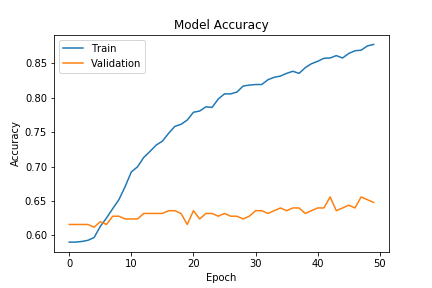
\includegraphics[scale=0.7]{subtask_b_first_gen_model_accuracy.png}
\end{figure}

\begin{figure}[H]
\caption{Strata sieci syjamskiej.\label{fig:suktecznoscbloss}}
\centering
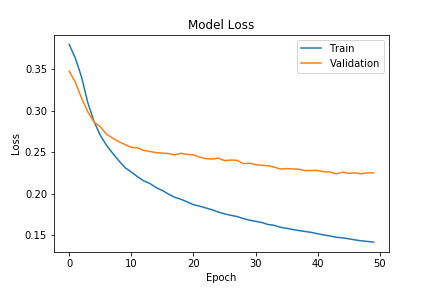
\includegraphics[scale=0.7]{subtask_b_first_gen_model_loss.png}
\end{figure}

Na powyższych wykresach (rysunki~\ref{fig:suktecznoscbacc} i \ref{fig:suktecznoscbloss}) widać, że po kilkunastu epokach doszło do przeuczenia sieci. W kolejnych epokach rosła dokładność na zbiorze treningowym, a dla zbioru walidującego utrzymywała się na tym samym poziomie. Ponieważ dokładność nie prezentuje pełnych informacji na temat wyuczonego modelu, w tablicy~\ref{tab:train_set_statistics_score_tableb}  przedstawione zostały jeszcze następujące miary: pokrycia, krzywa ROC (ang. \textit{Receiver operating characteristic}) i błędu pierwszego stopnia (ang. \textit{F1 score}).

\begin{table}[H]
\caption{Skuteczność sieci rekurencyjnej na zbiorze testowym.}
\label{tab:train_set_statistics_score_tableb}
    \begin{center}
        \begin{tabular}{ |c|c| } 
            \hline
            metryka & wartość\\
            \hline
            Accuracy & 0,639 \\
            \hline
            Precision & 0,312 \\
            \hline
            Recall & 0,625 \\ 
            \hline
            ROC curve & 0,634 \\ 
            \hline
            F1 score & 0,417 \\ 
            \hline
        \end{tabular}
    \end{center}
\end{table}

\subsubsection{Rezultaty dla rozszerzonego zbioru danych}

Jednym z najlepszych sposobów na pozyskanie lepszych wyników jest często zebranie większej ilości danych. W tym celu można skorzystać z innych, otwartych zbiorów danych w internecie. Niestety, takie zbiory mogą różnić się jakością i ostatecznie doprowadzić do pogorszenia wyników, dlatego zastosowano alternatywne podjeście. Kolejne pary były generowane dzięki zaobserwowaniu prostej zależności: nowe pytania o identycznej skali podobieństwa względem istniejącego pytania i występujące we wspólnym wątku powinny utworzyć nową parę o takiej samej istotności.
Zmodyfikowane zbiory miały następujący rozkład klas:

\begin{table}[H]
\caption{Rozkład klas w rozszerzonym zbiorze treningowym.}
\label{subtask_b_original_set_statistics_score_table}
    \begin{center}
        \begin{tabular}{ |c|c| } 
            \hline
            ,,Relevant'' & 31,55\% \\
            \hline
            ,,Irrelevant'' & 68,45\% \\ 
            \hline
        \end{tabular}
    \end{center}
\end{table}

\begin{table}[H]
\caption{Rozkład klas w rozszerzonym zbiorze testowym.}
\label{subtask_b_original_set_statistics_score_table}
    \begin{center}
        \begin{tabular}{ |c|c| } 
            \hline
            ,,Relevant'' & 30,48\% \\
            \hline
            ,,Irrelevant'' & 69,52\% \\ 
            \hline
        \end{tabular}
    \end{center}
\end{table}

Zachowane zostały proporcje klas, nadal najwięcej jest par o niskim podobieństwie.
Zbiór treningowy składał się z 9000, a testowy z 2395 par pytań.

\begin{figure}[H]
\caption{Skuteczność sieci syjamskiej po rozszerzeniu zbioru danych.}
\centering
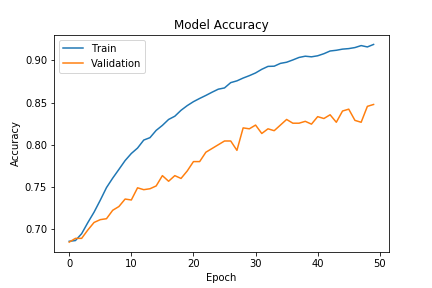
\includegraphics[scale=0.7]{subtask_b_second_gen_model_accuracy.png}
\end{figure}

\begin{figure}[H]
\caption{Strata sieci syjamskiej po rozszerzeniu zbioru danych.}
\centering
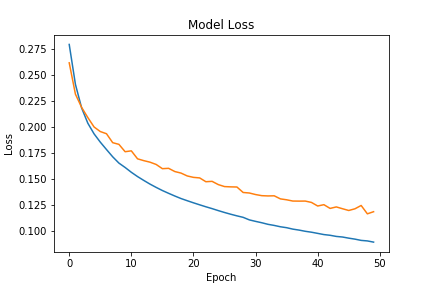
\includegraphics[scale=0.7]{subtask_b_second_gen_model_loss.png}
\end{figure}

\begin{table}[H]
\caption{Skuteczność sieci rekurencyjnej na zbiorze testowym.}
\label{train_set_statistics_score_table}
    \begin{center}
        \begin{tabular}{ |c|c| } 
            \hline
            metryka & wartość\\
            \hline
            Accuracy & 0,846 \\
            \hline
            Precision & 0,838 \\
            \hline
            Recall & 0,699 \\ 
            \hline
            ROC curve & 0,824 \\ 
            \hline
            F1 score & 0,771 \\ 
            \hline
        \end{tabular}
    \end{center}
\end{table}

\subsection{Ocena rezultatów}
Analizując wyniki otrzymane po wyuczeniu sieci syjamskich można stwierdzić, że rozszerzenie zbioru danych miało pozytywny wpływ na jakość klasyfikatora. Stworzenie nowych przykładów uczących zmieniło co prawda rozkład klas w zbiorze treningowym dla ,,Relevant'' z 40,8\% na 31,5\% i ,,Irrelevant'' z 59,2\% na 68,5\%, jednakże w tym samym czasie zaobserwowano wzrost m.in. dokładności sieci z 63,9\% na 84,6\%. 

\section{Podzadanie C}
\subsection{Analiza danych}
\subsubsection{Rozkład wartości etykiety}

Podzadanie C dotyczyło podobieństwa nowych pytań do istniejących komentarzy.  Każdy komentarz w zbiorze zawierał etykietę RELC\_RELEVANCE2ORGQ, która określała to podobieństwo. Etykieta przyjmowała trzy wartości: ,,Good'', ,,PotentiallyUseful'' oraz ,,Bad''. Rozkład etykiet w oryginalnym zbiorze przedstawiono w tablicy~\ref{c_original_set_percentage}.

\begin{table}[H]
\caption{Rozkład ilościowy klas w oryginalnym zbiorze.}
\label{c_original_set_percentage}
    \begin{center}
        \begin{tabular}{ |c|c| } 
            \hline
            ,,Good'' & 9,95\% \\
            \hline
            ,,PotentiallyUseful'' & 8,44\% \\
            \hline
            ,,Bad'' & 81,61\% \\ 
            \hline
        \end{tabular}
    \end{center}
\end{table}

Ze względu na sprowadzenie problemu do decyzji binarnej, klasa ,,PotentiallyUseful'' była traktowana jako część klasy ,,Good''. Tablica \ref{c_merged_set_percentage} pokazuje rozkład po złączeniu klas.

\begin{table}[H]
\caption{Rozkład ilościowy klas po połączeniu.}
\label{c_merged_set_percentage}
    \begin{center}
        \begin{tabular}{ |c|c| } 
            \hline
            ,,Good'' & 18,39\% \\
            \hline
            ,,Bad'' & 81,61\% \\ 
            \hline
        \end{tabular}
    \end{center}
\end{table}

\subsubsection{Sprawdzenie podobieństwa dla podstawowych miar}

Kolejnym etapem analizy danych było sprawdzenie powiązania między wartościami podstawowych miar podobieństwa a faktycznym podobieństwem, które było opisane w zbiorze danych za pomocą etykiety.

Rysunek~\ref{c_jaccard_distance} przedstawia medianę odległości Jaccarda dla obu klas w zbiorze. Dodatkowo na wykresie widać wartość pierwszego i trzeciego kwartyla oraz minimum i maksimum przyjmowanych wartości.

\begin{figure}[H]
\centering
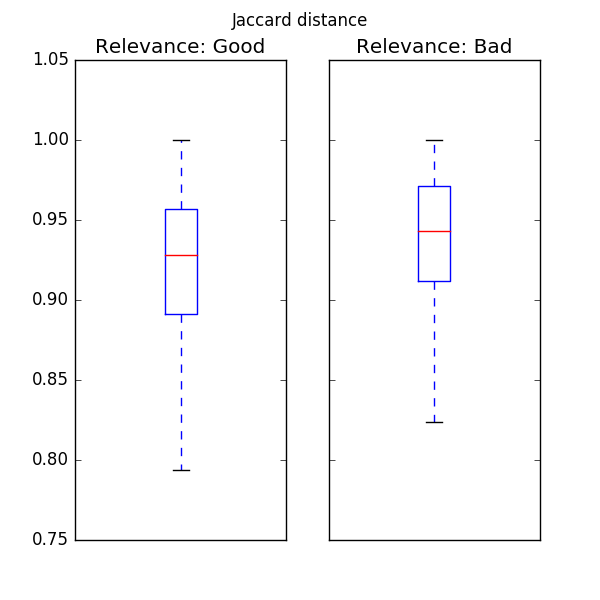
\includegraphics[scale=0.5]{c_Jaccard_distance.png}
\caption{Odległość Jaccarda.}
\label{c_jaccard_distance}
\end{figure}

Niestety otrzymane wyniki nie pozwalają na wyznaczenie wartości odległości Jaccarda, która oddzieliłaby skutecznie obie klasy. Miara ta bada podobieństwo jedynie na podstawie liczby tych samych słów użytych w porównywanych tekstach. Przykłady z klasy ,,Bad'', mimo różnicy znaczeniowej pytań i komentarzy, otrzymują wysokie wyniki, ponieważ w tekstach pojawiają się te same słowa.

Kolejną badaną miarą było podobieństwo cosinusowe. Wyniki przedstawia rysunek~\ref{c_cosine_similarity}.

\begin{figure}[H]
\centering
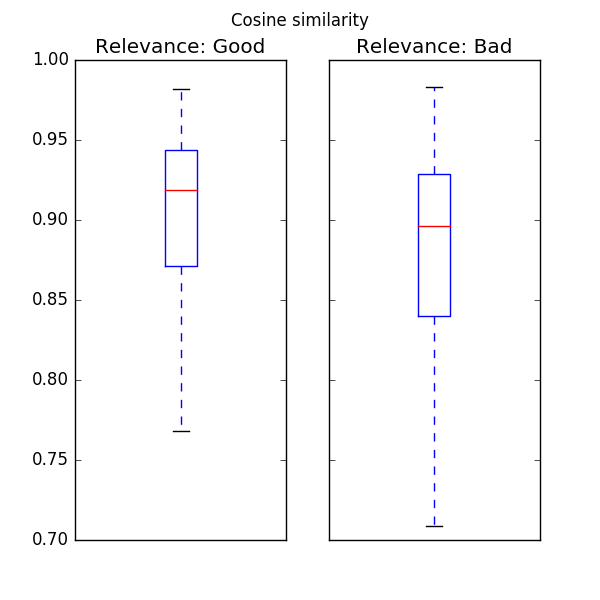
\includegraphics[scale=0.5]{c_Cosine_similarity.png}
\caption{Podobieństwo cosinusowe.}
\label{c_cosine_similarity}
\end{figure}

Choć w tym przypadku rozbieżność mediany dla klas jest nieco większa, nadal nie jest możliwe jednoznaczne rozdzielenie ze względu na podobne rozstępy międzykwartylowe. Wartości ponownie rozkładają się zbyt blisko siebie.

Rysunek~\ref{c_length_difference} przedstawia wyniki dla prostego badania różnicy długości.

\begin{figure}[H]
\centering
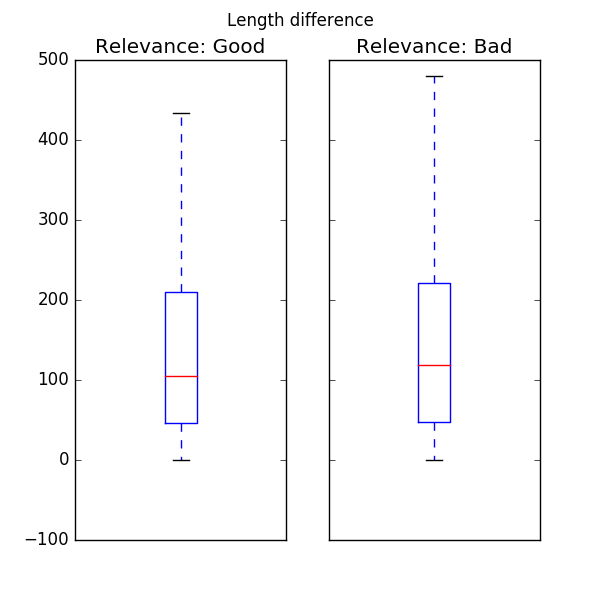
\includegraphics[scale=0.5]{c_Length_difference.png}
\caption{Różnica długości.}
\label{c_length_difference}
\end{figure}

W przypadku tej miary ponownie widać duże podobieństwo wyników dla obu klas. Wyniki pozwalają wręcz wnioskować, że w całym zbiorze danych różnica długości dla między pytaniem a komentarzem oscyluje w granicach 100 znaków. Niestety dla badania pobobieństwa miara różnicy długości nie była pomocna.

\subsection{Reprezentacja w postaci word embeddingów}
Ze względu na niską skuteczność podstawowych miar postanowiono użyć bardziej złożonych modeli klasyfikujących -- sieci neuronowych. Aby w pełni wykorzystać możliwości sieci do znajdowania wzorców, jako reprezentacje słów zostały wykorzystane \textit{word embeddingi}. Użyto zbioru wektorów udostępnianego przez firmę Google.

\subsection{Prosta sieć neuronowa (feed-forward)}

Pierwszy model sieci neuronowej jaki został przetestowany opierał się na prostej architekturze z jedną warstwą ukrytą o rozmiarze 128 jednostek. Ponieważ przygotowane próbki danych składały się z par pytanie-odpowiedź, sieć posiadała dwa wejścia. Każde z wejść było połączone z warstwą \textit{embedding}, czyli warstwą konwertującą dane wejściowe na reprezentacje wektorowe. Wektory wyjściowe były następnie łączone w jeden w warstwie konkatenacji. Połączony wektor trafiał do warstwy prostej, złożonej ze 128 neuronów. Ostatnią warstwę stanowił pojedynczy neuron wyjściowy.

Tak zbudowaną sieć wytrenowano w procesie trwającym 400 epok. Rysunki~\ref{c_feedforward_acc} oraz \ref{c_feedforward_loss} przedstawiają uzyskane wyniki.

\begin{figure}[H]
\centering
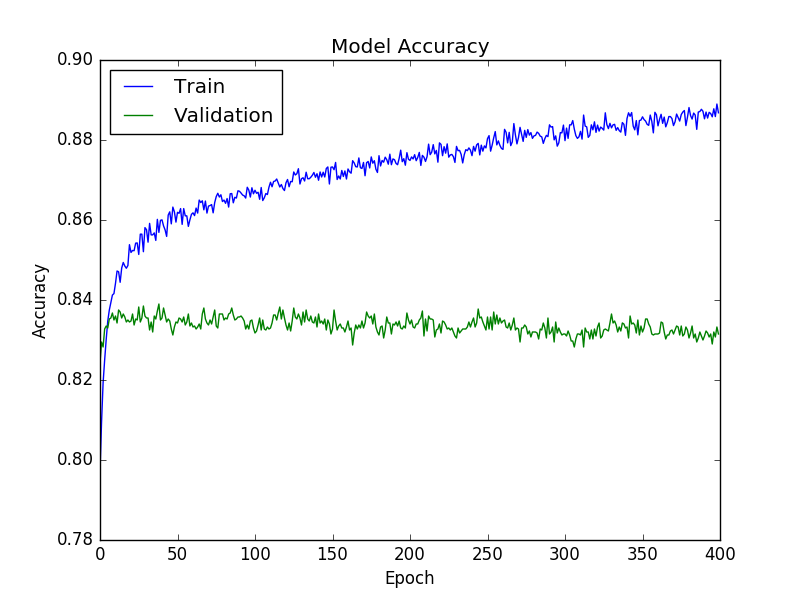
\includegraphics[scale=0.5]{c_feedforward_1_dense_128_acc.png}
\caption{Trafność sieci prostej.}
\label{c_feedforward_acc}
\end{figure}

\begin{figure}[H]
\centering
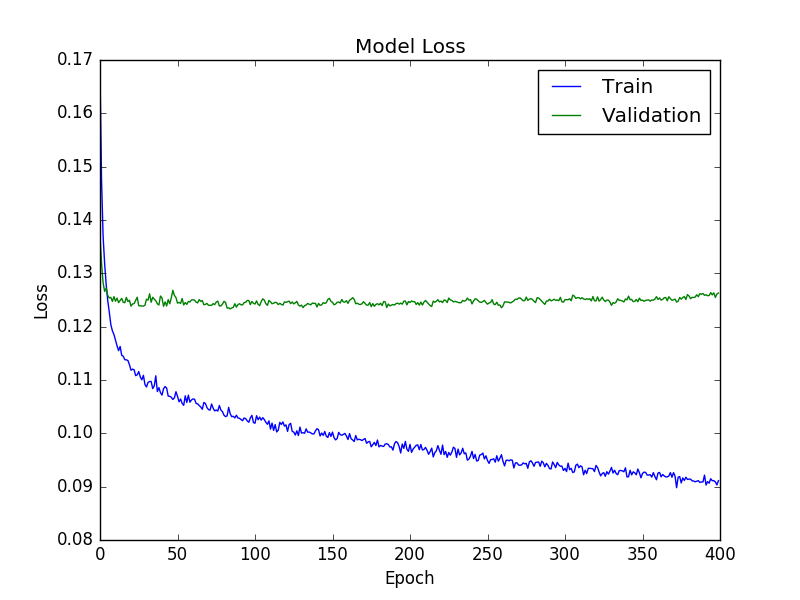
\includegraphics[scale=0.5]{c_feedforward_1_dense_128_loss.png}
\caption{Strata sieci prostej.}
\label{c_feedforward_loss}
\end{figure}

Choć na zbiorze trenującym sieć osiąga wysoką trafność, a błąd jest niewielki, na zbiorze walidującym wyniki nie ulegają znacznej poprawie w trakcie uczenia. Zarówno trafność jak i strata oscylują w granicach wartości uzyskanych w początkowych etapach treningu. W przypadku trafności można zauważyć nawet trend spadkowy. Są to objawy przeuczenia sieci, czyli zbyt silnego uzależnienia od przypadków ze zbioru trenującego.

\subsection{Sieci rekurencyjne}
\subsubsection{Sieć LSTM}

Zostały wytrenowane dwa modele sieci oparte o warstwę rekurencyjną \emph{Long Short-Term Memory} (LSTM). Warstwa w obu przypadkach miała rozmiar 128 jednostek. Model pierwszy składał się dodatkowo z warstwy prostej o tej samej wielkości i z jednego neuronu stanowiącego wyjście sieci. Wyniki przedstawiają rysunki~\ref{c_lstm_1_acc} oraz \ref{c_lstm_1_loss}.

\begin{figure}[H]
\centering
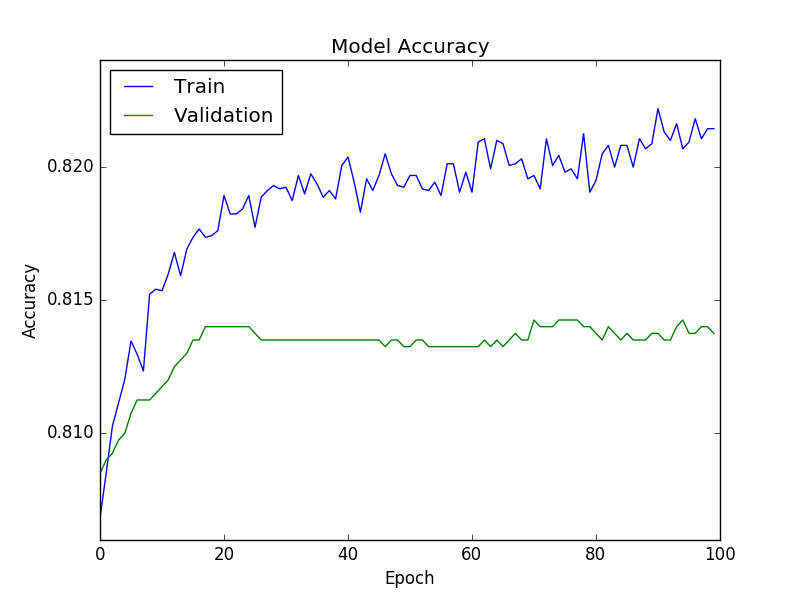
\includegraphics[scale=0.5]{c_lstm_1_dense_acc.png}
\caption{Trafność pierwszego modelu.}
\label{c_lstm_1_acc}
\end{figure}

\begin{figure}[H]
\centering
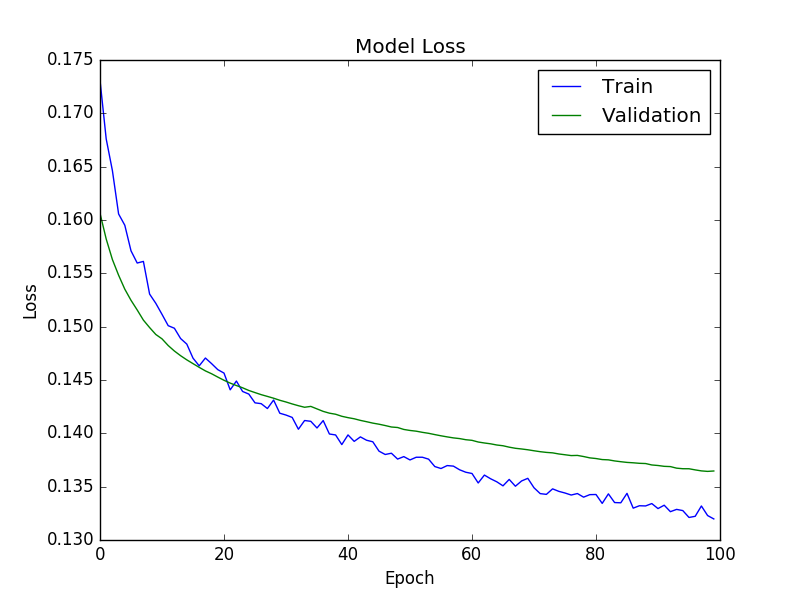
\includegraphics[scale=0.5]{c_lstm_1_dense_loss.png}
\caption{Strata pierwszego modelu.}
\label{c_lstm_1_loss}
\end{figure}

Wyniki wskazują na lekką poprawę w porównaniu z siecią prostą. Po wprowadzeniu warstwy rekurencyjnej sieć osiąga wynik trafności w granicach 81,5\% i nie wykazuje trendu spadkowego w trakcie uczenia. Mimo, że trafność na zbiorze trenującym jest nieco wyższa, strata modelu na obu zbiorach jest zbliżona i zachowała trend malejący. Sieć oparta na jednej warstwie prostej i jednej warstwie rekurencyjnej nie została przeuczona.

Model drugi wykorzystywał poza warstwą rekurencyjną, dwie warstwy proste o rozmiarach 128 i 64 jednostek oraz pojedynczy neuron wyjściowy. Wyniki uczenia przedstawiono na rysunkach~\ref{c_lstm_2_acc} oraz \ref{c_lstm_2_loss}.

\begin{figure}[H]
\centering
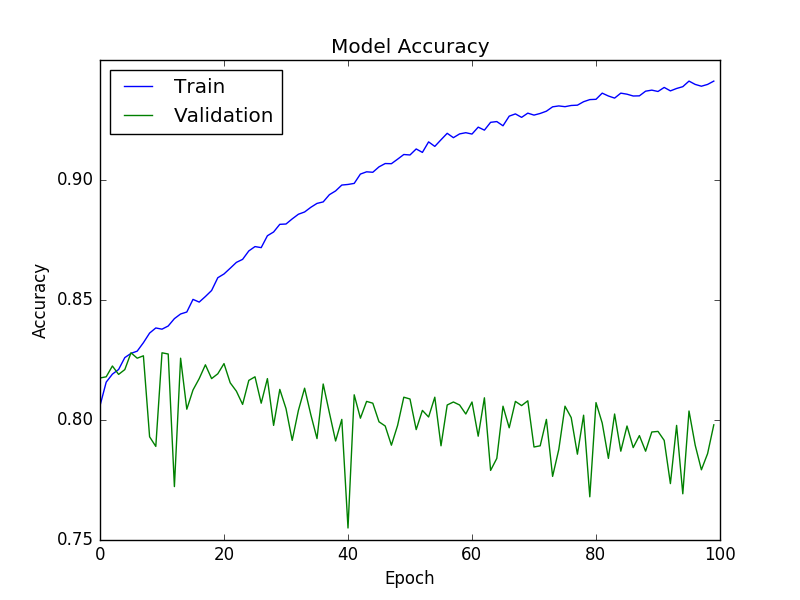
\includegraphics[scale=0.5]{c_lstm_3_dense_acc.png}
\caption{Trafność drugiego modelu.}
\label{c_lstm_2_acc}
\end{figure}

\begin{figure}[H]
\centering
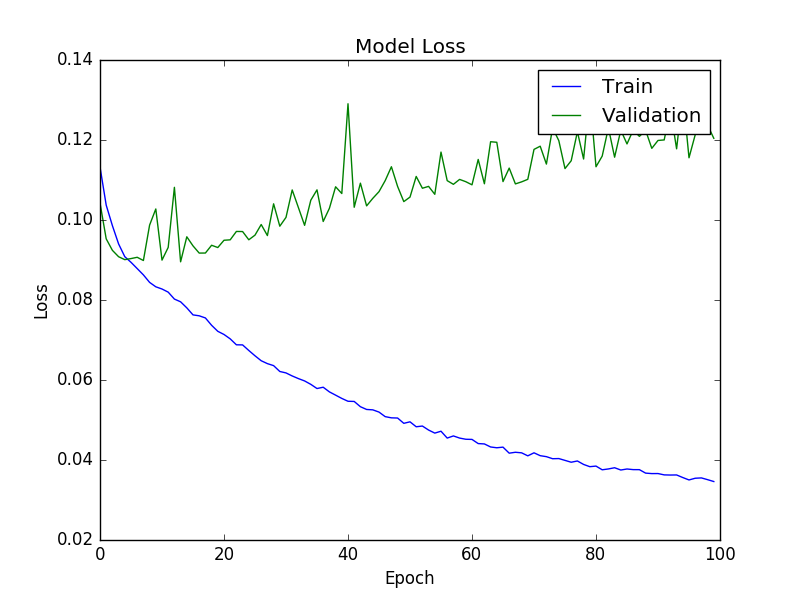
\includegraphics[scale=0.5]{c_lstm_3_dense_loss.png}
\caption{Strata drugiego modelu.}
\label{c_lstm_2_loss}
\end{figure}

Choć po kilku pierwszych epokach model ma zbliżone wyniki na obu zbiorach, szybko następuje przeuczenie. Na zbiorze walidującym trafność spada, a strata rośnie. Prawdopodobnie jest to spowodowane wprowadzeniem dodatkowej warstwy prostej. Po analizie wyników dla sieci feed-forward można wnioskować, że to tego typu warstwy są wrażliwe na przeuczenie. Aby uzyskać model nieprzeuczony, osiągający skuteczność ok. 82\% należałoby zatrzymać proces uczenia już po pięciu epokach.

\subsubsection{Sieć MaLSTM}
W celu dalszego poprawienia wyników stworzona została sieć syjamska w wariancie ogólnym. Model składał się z dwóch podsieci zawierających po jednej warstwie rekurenyjnej Long Short-Term Memory. Każda z nich o rozmiarze 128 jednostek. Dla wektorów na wyjściach obu podsieci była następnie obliczana norma w metryce manhatańskiej. Obliczona wartość trafiała do pojedynczego neuronu, który stanowił wyjście sieci.

Wyniki dot. trafności i straty przedstawiają rysunki~\ref{c_siamese_acc} i \ref{c_siamese_loss}.

\begin{figure}[H]
\centering
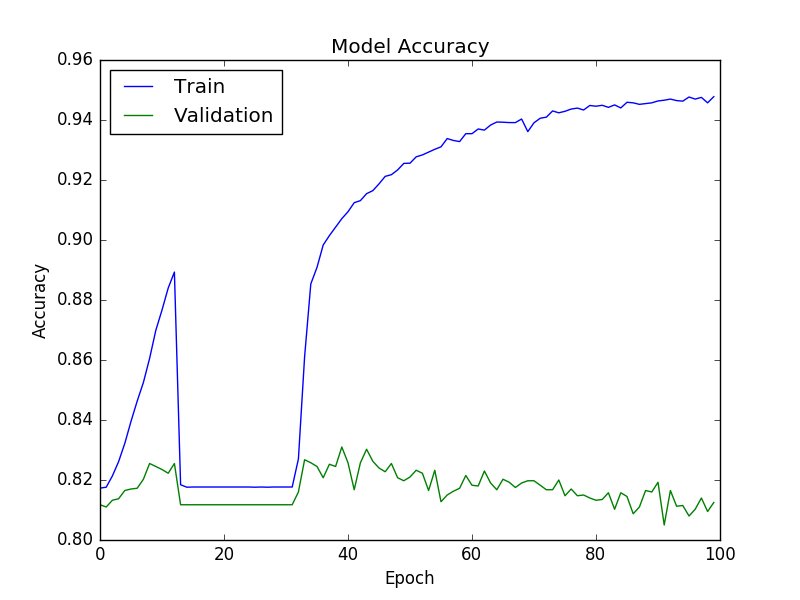
\includegraphics[scale=0.5]{c_malstm_org_dataset_acc.png}
\caption{Trafność sieci syjamskiej.}
\label{c_siamese_acc}
\end{figure}

\begin{figure}[H]
\centering
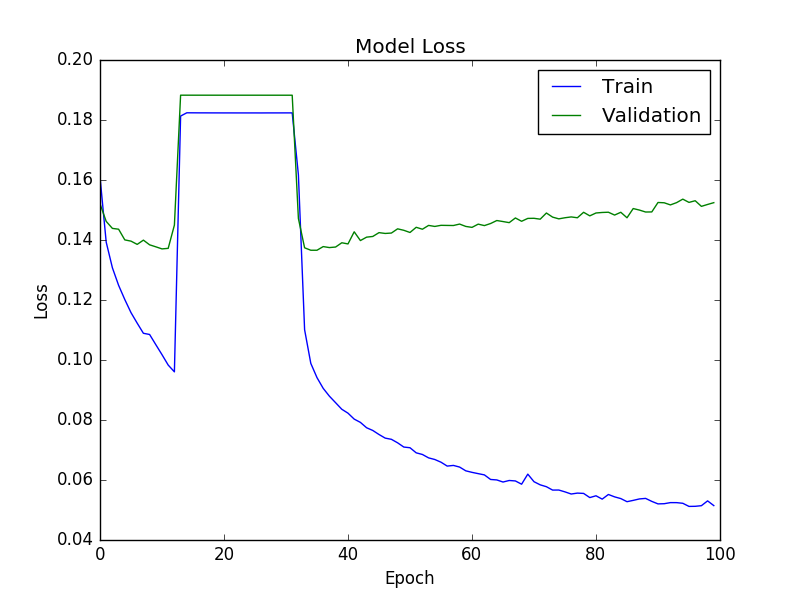
\includegraphics[scale=0.5]{c_malstm_org_dataset_loss.png}
\caption{Strata sieci syjamskiej.}
\label{c_siamese_loss}
\end{figure}

Wyraźnie widać, że w trakcie uczenia wystąpiła anomalia. Od epoki 15, przez ok. 20 epok zarówno trafność jak i strata na obu zbiorach mają stałe wartości. Prawdopodobnie przez ten okres wartości wag nie były w ogóle zmieniane. W dalszej części uczenia widać, że po raz kolejny wystąpiło przeuczenie, ponieważ mimo wzrostu trafności na zbiorze trenującym, trafność na zbiorze walidującym spadała. Podobnie strata, choć malała na zbiorze trenującym, rosła w przypadku zbioru walidującego. W najlepszym momencie sieć syjamska osiągnęła wynik niewiele ponad 82\% trafności.

\subsubsection{Rozszerzenie zbioru danych}

Jednym ze sposobów poprawy skuteczności modelu jest wytrenowanie go na większym zbiorze danych. W przypadku zbiorów dla uczenia nadzorowanego, warto również zwrócić uwagę na rozkład ilościowy poszczególnych klas. Dla podzadania C rozkład nie jest równy, ponieważ około 80\% przypadków należy do tej samej klasy.

Na podstawie oryginalnego zbioru został stworzony zbiór rozszerzony, w którym nowe próbki utworzono zamieniając niektóre wyrazy na ich synonimy. Dodatkowo, w celu wyrównania liczności klas, rozszerzeniu podlegały tylko próbki należące do klasy ,,Good''. Dokładną charakterystykę zbioru oryginalnego i rozszerzonego przedstawia tablica~\ref{c_augmented_set_percentage}.

\begin{table}[H]
\caption{Rozkłady ilościowe klas w zbiorze oryginalnym i rozszerzonym.}
\label{c_augmented_set_percentage}
    \begin{center}
        \begin{tabular}{ |c|c|c|c| } 
            \hline
            Zbiór & Liczność zbioru & ,,Good'' & ,,Bad''\\
            \hline
            Oryginalny & 19954 & 18,38\% & 81,61\%\\
            \hline
            Rozszerzony & 40370 & 59,66\% & 40,34\%\\ 
            \hline
        \end{tabular}
    \end{center}
\end{table}

Na zbiorze rozszerzonym został wytrenowany model sieci syjamskiej. Wyniki przedstawiają rysunki~\ref{c_siamese_augmented_acc} i \ref{c_siamese_augmented_loss}.

\begin{figure}[H]
\centering
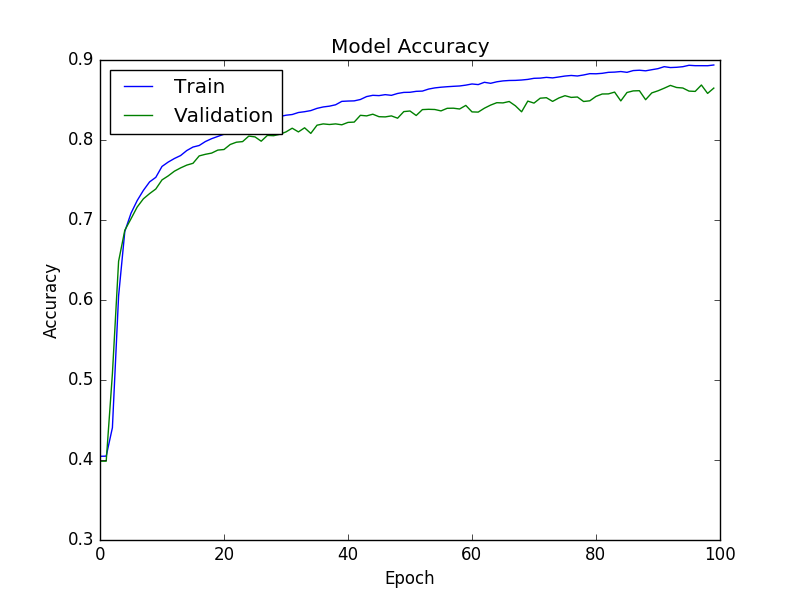
\includegraphics[scale=0.5]{c_siamese_augmented_dataset_acc.png}
\caption{Trafność sieci syjamskiej na zbiorze rozszerzonym.}
\label{c_siamese_augmented_acc}
\end{figure}

\begin{figure}[H]
\centering
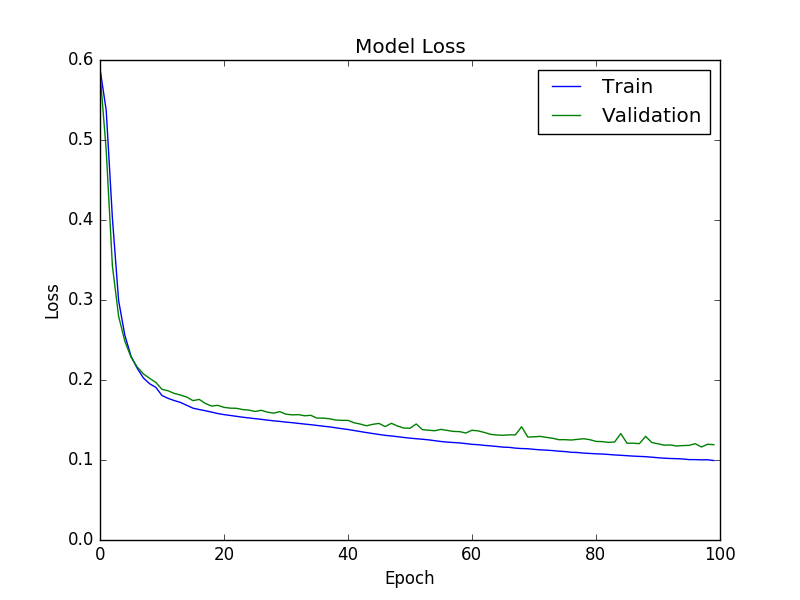
\includegraphics[scale=0.5]{c_siamese_augmented_dataset_loss.png}
\caption{Strata sieci syjamskiej na zbiorze rozszerzonym.}
\label{c_siamese_augmented_loss}
\end{figure}

Trafność działania modelu na zbiorze walidującym została zwiększona, osiągnęła ostatecznie wynik około 85\%.

\subsection{Ocena rezultatów}
Warto rozważyć otrzymane wyniki w oparciu o rozkład danych. W zbiorze oryginalnym ok. 80\% stanowiły przykłady z klasy ,,Bad''. Oznacza to, że klasyfikator, który dla każdej pary pytanie-odpowiedź zwracałby klasę ,,Bad'' osiągałby poziom trafności w granicach 80\%. Model sieci syjamskiej wytrenowany na oryginalnym zbiorze osiągnął trafność ok. 82\%. Wynik ten, choć na pierwszy rzut oka wysoki, nie przewyższa zanadto wyniku, który mógłby osiągnąć naiwny klasyfikator zwracający zawsze tą samą klasę. Poprawę trafności widać dopiero po wytrenowaniu tej samej sieci syjamskiej na zbiorze rozszerzonym. W tej wersji zbioru rozkład klas jest bardziej równomierny, naiwny klasyfikator mógłby osiągnąć na nim co najwyżej trafność ok. 60\%, ponieważ taką część zbioru stanowi klasa ,,Good''. Sieć syjamska osiąga trafność na poziomie 85\%.
\section{Podzadanie E}
\subsection{Analiza danych}
\subsubsection{Format danych}

Format danych w tym podzadaniu jest wzbogacony o dodatkowe atrybuty dla znaczników XML: ,,RelQuestion'', ,,RelAnswer'' oraz ,,RelComment''. Umożliwia to pobranie większej liczby miar statystycznych niż w poprzednich przypadkach.

Element \emph{,,RelQuestion''} zawiera dodatkowe pola tj.: \emph{liczba punktów} czy \emph{liczba wyświetleń}. Są one wykorzystane przy sprawdzaniu miar statystycznych. Struktura tego elementu przedstawia się następująco:

\begin{lstlisting}[language=XML,breaklines,label={lst:subtask_e_rel_question},caption={Przykład elementu ,,RelQuestion''.}]
<RelQuestion RELQ_CATEGORY="cooking" RELQ_DATE="2015-09-28 12:36:51" RELQ_ID="236203783777_R223248892008" RELQ_RANKING_ORDER="1" RELQ_RELEVANCE2ORGQ="Irrelevant" RELQ_SCORE="1" RELQ_TAGS="indian-cuisine, texture" RELQ_USERID="39650" RELQ_USERNAME="" RELQ_VIEWCOUNT="82">
  <RelQSubject>
    Remedy for Dry Chicken Yakhni pulao ?
  </RelQSubject>
  <RelQBody>
    My question is that today I prepared Chicken Yakhni Pulao,it tasted good but it is very dry, i mean the youghurt and the masala got absorbed in the rice very much. And i have made lots of it, it is also fully cooked. So does anyone know how should i make the fully cooked pulao little juicy ? As it is difficult to eat the dry pulao(I may require another curry with it)
  </RelQBody>
</RelQuestion>
\end{lstlisting}

Element \emph{,,RelAnswer''} zawiera kilka dodatkowych atrybutów. Nie zostały one jednak wykrzystane w późniejszych eksperymentach. Struktura tego elementu przedstawia się następująco:

\begin{lstlisting}[language=XML,breaklines,label={lst:subtask_e_rel_answer},caption={Przykład elementu ,,RelAnswer''.}]
<RelAnswer RELA_ACCEPTED="0" RELA_DATE="2015-09-29 10:44:51" RELA_ID="236203783777_R223248892008_A506889689755" RELA_RELEVANCE2ORGQ="" RELA_RELEVANCE2RELQ="" RELA_SCORE="0" RELA_USERID="37725" RELA_USERNAME="">
  <RelAText>
    I recon it has formed like a cake after cooling. The best option you have is to take a big chunk of it in a microwaveable container (making sure that you are not breaking the rice grains) and sprinkling with some water. Then cover with a cling film and microwave for 3-4 minutes from cold. Your rice grains will separate because of the extra moisture from the sprinkled water and the Pulao will become slightly moist.   But yes, Pulao is a dry dish and needs to be eaten with a side like Raita or Salan.
  </RelAText>
</RelAnswer>
\end{lstlisting}

Podobnie jak poprzedni element, \emph{,,RelComment''} zawiera dodatkowe atrybuty, lecz nie zostały one wykorzystane. Struktura tego elementu wygląda w następujący sposób:

\begin{lstlisting}[language=XML,breaklines,label={lst:subtask_e_rel_comment},caption={Przykład elementu ,,RelComment''.}]
<RelComment RELC_DATE="2015-09-29 11:57:05" RELC_ID="236203783777_R223248892008_C246533537180" RELC_RELEVANCE2ORGQ="" RELC_RELEVANCE2RELQ="" RELC_SCORE="1" RELC_USERID="17272" RELC_USERNAME="">
  <RelCText>
    Are you trying to make it better next time, or salvage what you've already made?
  </RelCText>
</RelComment>
\end{lstlisting}

\subsubsection{Rozkład danych}
Podzadanie E miało na celu stwierdzenie czy dane pytanie jest duplikatem. Polega to na porównaniu przykładowego pytania z pytaniem istniejącym już na forum dyskusyjnym, które zawiera również wątek odpowiedzi oraz komentarzy. Zbiór danych pochodzi z forum ,,Stack Exchange - English Language''.
Oryginalny zbiór zawiera \emph{1035065 par pytań}, a jego rozkład danych przedstawia się następująco:

\begin{table}[H]
\caption{Rozkład klas w zbiorze uczącym.}
\label{se_train_set_unmodified}
    \begin{center}
        \begin{tabular}{ |c|c| } 
            \hline
            klasa & rozkład\\
            \hline
            PerfectMatch & 0,0468\% \\
            \hline
            Related & 0,7201\% \\
            \hline
            Irrelevant & 99,232\% \\
            \hline
        \end{tabular}
    \end{center}
\end{table}

W oryginalnym zbiorze danych przeważają przykłady oznaczone etykietą ,,Irrelevant''. Jest to problem, ponieważ nie pozwala to na poprawne wyuczenie sieci neuronowej. Rozwiązaniem tego problemu, może być dogenerowanie przykładów z etykietą ,,PerfectMatch''. Po modyfikacji zbioru danych, rozmiar zredukował się do \emph{30407 elementów}, a jego rozkład przedstawia się w taki sposób:

\begin{table}[H]
\caption{Rozkład klas w zmodyfikowanym zbiorze uczącym.}
\label{se_train_set_modified}
    \begin{center}
        \begin{tabular}{ |c|c| }
            \hline
            klasa & rozkład\\
            \hline
            PerfectMatch & 25,1619\% \\
            \hline
            Related & 24,5140\% \\
            \hline
            Irrelevant & 50,3239\% \\
            \hline
        \end{tabular}
    \end{center}
\end{table}

Udział klasy ,,PerfectMatch'' w zbiorze treningowym wynosi około 25\%, co~pozwala na dużo lepsze wyuczenie sieci neuronowej mimo zredukowanego rozmiaru zbioru uczącego.

Zadanie polega na stwierdzeniu czy pytanie jest duplikatem istniejącego już pytania, a wyłącznie etykieta ,,PerfectMatch'' odpowiada takiemu zdarzeniu, można więc zredukować zbiór danych do 2 klas: \emph{Duplicate} oraz \emph{Non-duplicate}. Rozkład klas przedstawia się wtedy następująco:

\begin{table}[H]
\caption{Rozkład zredukowanych klas w zbiorze uczącym.}
\label{se_train_set_reduced}
    \begin{center}
        \begin{tabular}{ |c|c| }
         \hline
         klasa & rozkład \\
         \hline
         Duplicate & 25,1619\% \\
         \hline
         Non-duplicate & 74,8381\% \\
         \hline
        \end{tabular}
    \end{center}
\end{table}

\subsection{Miary statystyczne}

Podobnie jak w przypadku poprzednich podzadań, pierwszą próbą rozwiązania tego problemu, było porównanie miar statystycznych dwóch tekstów w celu sprawdzenia podobieństwa między nimi. Istnieje jednak różnica między poprzednimi podzadaniami. W zbiorze danych dla podzadania E zostały dodane dodatkowe atrybuty. Problem z nierównością rozkładu klas nie dotyczy badań miar statystycznych, dlatego skorzystano z danych o rozkładzie przedstawionym w tablicy~ \ref{se_train_set_unmodified}. Wykonano jednak połączenie klas ,,Irrelevant'' oraz ,,Related'' w jedną klasę ,,Non-duplicate''. Etykieta ,,PerfectMatch'' została zamieniona na ,,Duplicate''.

\begin{figure}[H]
\centering
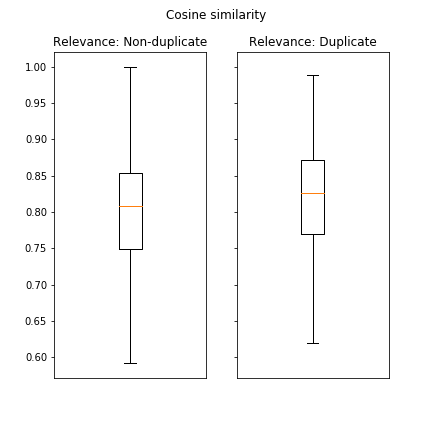
\includegraphics[scale=0.5]{e_en_train_cosine_similarity.png}
\caption{Zależność podobieństwa kosinusowego i klasy.}
\end{figure}

Porównując podobieństwa kosinusowe dla par tekstów oznaczonych etykietą ,,Duplicate'' oraz ,,Non-duplicate'' nie widać wyraźnej różnicy między wartościami mediany, pierwszego kwartylu ani trzeciego kwartylu. Dlatego na podstawie tej miary, nie jesteśmy w stanie stwierdzić podobieństwa między dwoma tekstami.

\begin{figure}[H]
\centering
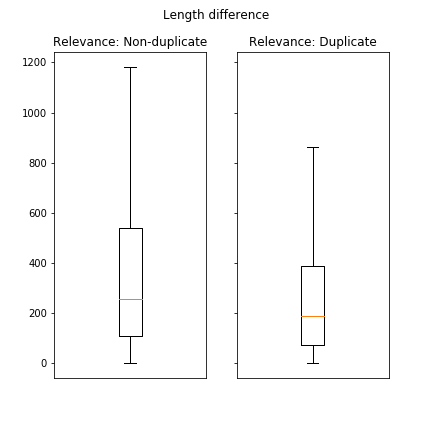
\includegraphics[scale=0.5]{e_en_train_length_difference.png}
\caption{Zależność różnicy długości i klasy.}
\end{figure}

Różnica długości dwóch tekstów, podobnie jak miara podobieństwa kosinusowego, nie jest w stanie sama określić podobieństwa między tymi tekstami.

\begin{figure}[H]
\centering
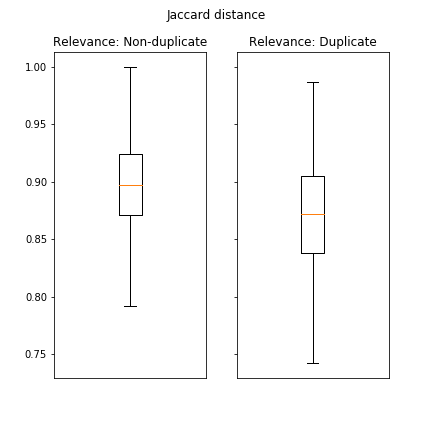
\includegraphics[scale=0.5]{e_en_train_jaccard_distance.png}
\caption{Zależność odległości Jaccarda i klasy}
\end{figure}

Dla większości par tekstów oznaczonych etykietą ,,Duplicate'', wartości znajdowały się w przedziale $\langle 0,85-0,92 \rangle$. Porównując to z wartościami dla par oznaczonych klasą ,,Non-duplicate'', nadal nie możemy stwierdzić które przypadki są duplikatami, a które nie.

Kolejne miary przedstawione na wykresach, są możliwe do wyznaczenia tylko w przypadku tego podzadania. Zbiór danych różni się atrybutami które są umieszczone w znacznikach XML. Wypróbowanych zostało 6 dodatkowych miar. Są to:

\begin{itemize}
\item liczba wyświetleń pytania powiązanego,
\item liczba punktów pytania powiązanego,
\item liczba odpowiedzi,
\item liczba komentarzy,
\item całkowita liczba głosów na odpowiedzi do pytania powiązanego,
\item liczba głosów na najlepszą odpowiedź do pytania powiązanego.
\end{itemize}

\begin{figure}[H]
    \begin{subfigure}{.5\textwidth}
        \label{fig:subtask_e_view_count}
        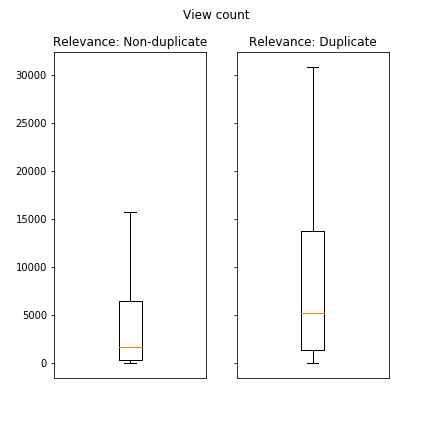
\includegraphics[width=\linewidth]{e_en_train_view_count.png}
        \caption{Liczba wyświetleń.}
    \end{subfigure}
    \begin{subfigure}{.5\textwidth}
        \label{fig:subtask_e_score}
        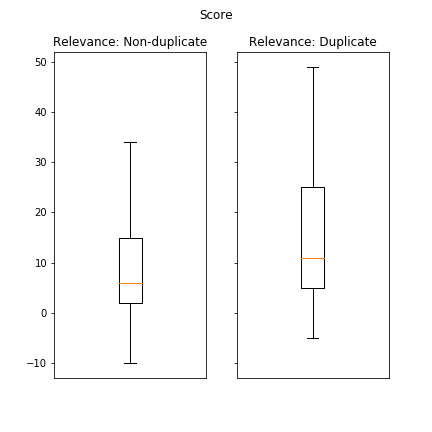
\includegraphics[width=\linewidth]{e_en_train_score.png}
        \caption{Liczba punktów.}
    \end{subfigure}
    \begin{subfigure}{.5\textwidth}
        \label{fig:subtask_e_no_of_answers}
        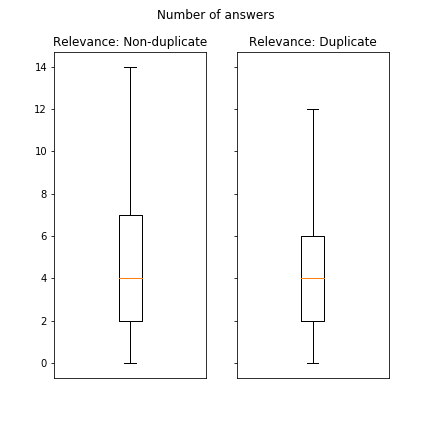
\includegraphics[width=\linewidth]{e_en_train_no_of_answers.png}
        \caption{Liczba odpowiedzi.}
    \end{subfigure}
    \begin{subfigure}{.5\textwidth}
        \label{fig:subtask_e_no_of_comments}
        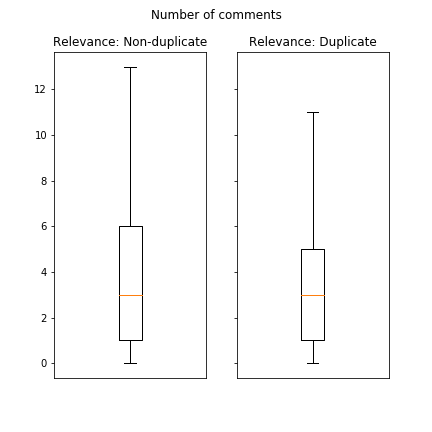
\includegraphics[width=\linewidth]{e_en_train_no_of_comments.png}
        \caption{Liczba komentarzy.}
    \end{subfigure}
    \begin{subfigure}{.5\textwidth}
        \label{fig:subtask_e_total_answer_upvotes}
        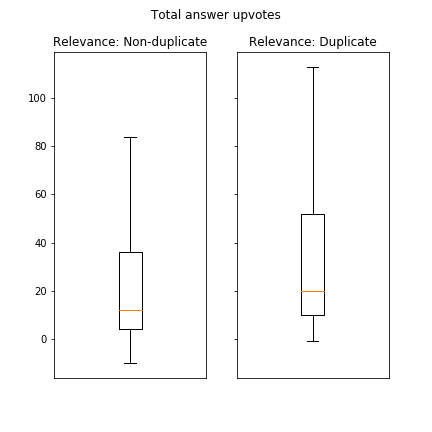
\includegraphics[width=\linewidth]{e_en_train_total_answer_upvotes.png}
        \caption{Liczba głosów na wszystkie odpowiedzi.}
    \end{subfigure}
    \begin{subfigure}{.5\textwidth}
        \label{fig:subtask_e_best_answer_upvotes}
        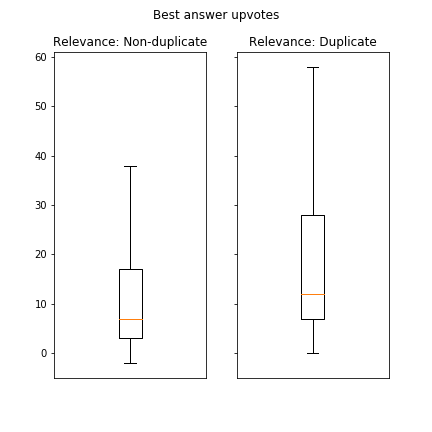
\includegraphics[width=\linewidth]{e_en_train_best_answer_upvotes.png}
        \caption{Liczba głosów na najlepszą odpowiedź.}
    \end{subfigure}
    \caption{Miary podobieństwa dla podzadania E.}
    \label{fig:e_multifigure}
\end{figure}

Powyższe wykresy (rysunki~\ref{fig:e_multifigure}) przedstawiają porównania miar statystycznych dla dwóch klas. Tak jak i w przypadku różnic długości tekstów, podobieństwa kosinusowego oraz indeksu Jaccarda, żadna z tych miar nie jest w stanie ocenić podobieństwa między dwoma tekstami.

\subsection{Sieci neuronowe}
\subsubsection{Przygotowanie danych}
Do wytrenowania sieci neuronowej wykorzystany został zbiór danych o rozkładzie przedstawionym w tablicy~\ref{se_train_set_modified}. Zbiór został podzielony na część treningową, z \emph{25407 parami tekstów}, oraz walidacyjną z \emph{5000}. Na potrzeby sieci neuronowej, etykiecie ,,Duplicate'' została przypisana wartość \emph{1}, natomiast ,,Non-duplicate'', wartość \emph{0}.

\subsubsection{Sieć syjamska}
Korzystając z eksperymentów przeprowadzonych na potrzeby poprzednich zadań, pierwszą próbą rozwiązania problemu znajdowania duplikatów za pomocą sieci neuronowych, było wykorzystanie architektury sieci syjamskich.
Architektura tej sieci została przedstawiona w rozdziale \ref{arch:malstm}. W warstwie rekurencyjnej zastosowanych zostało 50 ukrytych jednostek. Wykresy przebiegu uczenia sieci przedstawiają się następująco:

\begin{figure}[H]
\centering
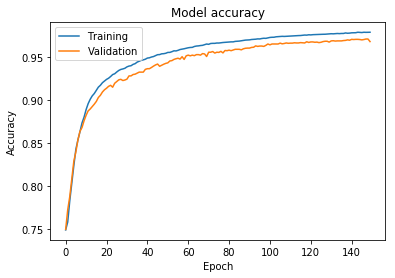
\includegraphics[scale=0.5]{e_malstm_acc.png}
\caption{Trafność sieci.}
\label{fig:e_malstm_acc}
\end{figure}

\begin{figure}[H]
\centering
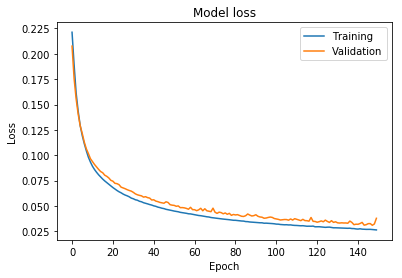
\includegraphics[scale=0.5]{e_malstm_loss.png}
\caption{Strata sieci.}
\label{fig:e_malstm_loss}
\end{figure}

Wykorzystany model sieci neuronowej sprawdził się bardzo dobrze na potrzeby tego zadania. Trafność sieci na zbiorze walidacyjnym na początku treningu wynosiła \emph{74,94\%}, natomiast po 150 epokach, wzrosła do \emph{96,84\%}. Strata w tym modelu, określona jako błąd średniokwadratowy, spadła z \emph{0,2075} do \emph{0,0308}.

\subsection{Ocena rezultatów}

Udział przeważającej klasy ,,Non-duplicate'' w zbiorze danych powoduje, że prosty klasyfikator oznaczający każdą parę zdań jako niezduplikowane miałby trafność na poziomie $\approx$~75\%. Ostateczny klasyfikator uzyskał jednak trafność $\approx$~97\%. Rozważając wyniki w oparciu o rozkład danych, można uznać, że model sieci syjamskiej potrafi z dużą dokładnością stwierdzić czy dwa teksty są swoimi duplikatami.


\chapter{Zakończenie}
Cele opisane we wstępie niniejszej pracy zostały osiągnięte. W ramach projektu została przyswojona podstawowa wiedza z zakresu przetwarzania języka naturalnego oraz budowy i działania modeli uczących, w szczególności sieci neuronowych. Zapoznano się również z narzędziami wykorzystywanymi do realizacji zadań związanych z tematyką pracy. Zdobyta wiedza została wykorzystana w praktyce do przeprowadzenia analizy zbioru danych oraz do stworzenia modeli klasyfikatorów spełniających wymagania czterech podzadań konkursu Sem-Eval. Modele zostały wytrenowane, a następnie przeanalizowane pod kątem skuteczności. Osiągnięto satysfakcjonujące wyniki, modele osiągały skuteczność powyżej 80\% przy zbliżonym rozkładzie ilościowym obu klas.

Podczas realizacji projektu napotkano problemy typowe dla zadań związanych z uczeniem maszynowym. Pierwszy z nich to brak wystarczającej mocy obliczeniowej. Wykorzystywane na początku laptopy i komputery stacjonarne nie posiadały zasobów sprzętowych pozwalających trenować sieci neuronowe w rozsądnym czasie. Konieczne było zwiększenie możliwości sprzętowych przez rozbudowanie komputerów lub skorzystanie z usług platform typu IaaS (Infrastructure as a Service). Drugim problemem była niewystarczająca ilość danych. Problem ten rozwiązano poprzez sztuczne powiększanie zbioru. Lepszym rozwiązaniem byłoby prawdopodobnie zdobycie prawdziwych danych, jednak ze względu na specyfikę projektu nie było to możliwe.

Ponieważ zadania konkursowe są inspirowane rzeczywistymi problemami, stworzone rozwiązania znajdują zastosowania w praktyce. Klasyfikatory porównujące pytania z komentarzami mogłyby posłużyć jako wsparcie dla użytkowników korzystających z forum typu Q\&A. Klasyfikatory badające podobieństwo pytań wsparłyby natomiast administratorów forum. Dostosowanie modeli do działania w ramach rzeczywistego forum otwiera ścieżki dla dalszego rozwoju projektu. Ze względu na ciągły przyrost treści na forum możnaby zaprojektować modele tak, aby było możliwe ich ,,douczanie'' na nowych przykładach (\emph{online learning}). W celu zwiększenia skuteczności możliwe byłoby również stworzenie łańcucha współpracujących klasyfikatorów. Przykładowo, klasyfikator znajdujący podobne pytania mógłby wspomóc działanie klasyfikatora dopasowującego odpowiedzi na nowe pytania.

% Bibliography (books, articles) starts here.
\bibliographystyle{plalpha}{\raggedright\sloppy\small\bibliography{bibliography}}

% Colophon is a place where you should let others know about copyrights etc.
\ppcolophon

\end{document}
